\documentclass{beamer}
\usetheme{AnnArbor}
\usecolortheme{seahorse}
% \usetheme{default}
% \usecolortheme{beaver}
\usepackage{graphicx}
\graphicspath{{pics/}}
\usepackage{amsmath}
\usepackage{amssymb}
\usepackage{framed}
\usepackage{tikz}
\usepackage[]{xcolor}
\usepackage[most]{tcolorbox}
\usepackage{pgfplots}
\pgfplotsset{compat=1.18}
\usepackage{blkarray}
\setbeamercolor{mycolorbox}{%
  bg=yellow!20,   % background color (20% yellow)
  fg=black      % foreground (text) color
}
\usefonttheme[onlymath]{serif}

\newtcolorbox{solutionblock}{
  colback=yellow!5,        % Background color: light yellow
  colframe=orange!80!black, % Frame color: dark orange
  title=Solution,
  fonttitle=\bfseries
}



%Information to be included in the title page:
\title{Algebra}
\author{Nithin}
\institute{Maveric Systems}
\date{\today}

\begin{document}
  \begin{frame}
    \titlepage
  \end{frame}

  \begin{frame}
    \tableofcontents
    \end{frame}

%  \section{Introduction}
\begin{frame}{Origins of Algebra}
    \begin{itemize}
      \item \textbf{Mesopotamia \& Egypt (c. 2000–1600 BCE)}
        \begin{itemize}
          \item Early problem-solving (linear/quadratic equations) in word problems
          \item No formal symbols, but systematic procedures
        \end{itemize}
  
      \item \textbf{Greek Era (c. 600 BCE–300 CE)}
        \begin{itemize}
          \item Geometric methods for solving equations (Euclid, Apollonius)
          \item Diophantus introduced proto-symbolic notation
        \end{itemize}
  
      \item \textbf{Islamic Golden Age (8th–12th Century)}
        \begin{itemize}
          \item Al-Khwarizmi’s work \emph{Al-jabr} $\rightarrow$ term “Algebra”
          \item Systematic solutions for linear and quadratic equations
        \end{itemize}
  
      \item \textbf{Transmission to Europe (12th–17th Century)}
        \begin{itemize}
          \item Latin translations influenced Fibonacci, others
          \item Viète, Descartes established modern symbolic notation \& analytic geometry
        \end{itemize}
  
      \item \textbf{Modern Algebra (19th–20th Century)}
        \begin{itemize}
          \item Emergence of abstract algebra (groups, rings, fields)
          \item Galois, Abel, and others formalized algebraic structures
        \end{itemize}
    \end{itemize}
  \end{frame}
  \begin{frame}{What is Algebra?}
    Algebra is a branch of mathematics that deals with numbers, variables, and their relationships. Key concepts include:
    \begin{itemize}
        \item \textbf{Variables}: Symbols (like \( x \), \( y \)) representing unknown or changing values.
        \item \textbf{Expressions}: Combinations of variables, numbers, and operations. E.g., \( 2x + 3 \).
        \item \textbf{Equations}: Mathematical statements that express equality, e.g., \( 2x + 3 = 7 \).
        \item \textbf{Solving Equations}: Finding values for variables that make an equation true.
        \item \textbf{Polynomials}: Expressions like \( 3x^2 + 2x - 5 \) involving variables raised to powers.
        \item \textbf{Functions}: Describes a relationship between variables, e.g., \( y = 2x + 1 \).
    \end{itemize}
\end{frame}
\begin{frame}{Why Algebra is Important in Machine Learning}
 
    \begin{itemize}
      \item \textbf{Data Representation:}  
      Data is often represented as vectors, matrices, and tensors. Algebra provides the tools for efficiently handling these structures.
      \item \textbf{Model Building:}  
      Many machine learning models (e.g., linear regression, neural networks) rely on algebraic operations like matrix multiplication and linear transformations.
      \item \textbf{Optimization:}  
      Training models involves solving systems of equations, computing gradients, and performing matrix decompositions, all of which require algebra.
      \item \textbf{Theoretical Insights:}  
      Concepts such as feature spaces, eigenvalues, eigenvectors, and dimensionality reduction (e.g., PCA) are based on algebraic principles.
      \item \textbf{Computational Efficiency:}  
      Algebraic methods enable the development of efficient algorithms that can be optimized for modern hardware.
    \end{itemize}
 
\end{frame}


  \begin{frame}{Integers}
    \begin{itemize}
        \item The set of integers is denoted by \(\mathbb{Z}\).
        \item Integers include:
        \[
          \ldots, -3, -2, -1, 0, 1, 2, 3, \ldots
        \]
        \item Formally, \(\mathbb{Z} = \{\dots, -2, -1, 0, 1, 2, \dots\}\).
        \item Common properties:
        \begin{itemize}
            \item \(\mathbb{Z}\) is infinite and unbounded in both the negative and positive directions.
            \item Closed under addition, subtraction, and multiplication:
                \[
                  \forall a, b \in \mathbb{Z}, \quad
                  a \pm b \in \mathbb{Z}, \quad
                  a \cdot b \in \mathbb{Z}.
                \]
        \end{itemize}
        \item The quotient of any two integers is not necessarily an integer. So we need to extend arithmetic to \textbf{rational numbers}
    \end{itemize}
\end{frame}
% Slide: Rational Numbers
\begin{frame}{Rational Numbers}
    \begin{itemize}
        \item The set of rational numbers is denoted by \(\mathbb{Q}\).
        \item Definition:
        \[
          \mathbb{Q} = \left\{ \frac{p}{q} \,\middle|\,
            p \in \mathbb{Z}, \; q \in \mathbb{Z}, \; q \neq 0
          \right\}.
        \]
        \item Every integer is also a rational number (e.g., \(5 = \frac{5}{1}\)).
        \item Examples:
        \[
          \frac{1}{2}, \quad -\frac{3}{4}, \quad 0, \quad 7, \quad \frac{11}{5}, \ldots
        \]
        \item Properties:
        \begin{itemize}
            \item Closed under addition, subtraction, multiplication, and division (except division by zero).
            \item Densely packed on the number line: between any two rationals, there is another rational.
        \end{itemize}
    \end{itemize}
\end{frame}
\begin{frame}
    \frametitle{Interesting Facts}
    \begin{itemize} 
        \item Why division by zero is prohibited ?
        \begin{itemize}
            \item Division is inverse of multiplication in the sense  
            \[  
            \frac{m}{n} \cdot n = m
            \]
        \item if \( n=0 \) and \( m = 1\), we get \(\frac{1}{0} \cdot 0 = 1\) which is nonsensical as any number multiplied by zero is zero
        \end{itemize}
        \item Rational numbers suffice for all actual physical measurements like weight, height and length
        \item But Geometry, Algebra and Calculus force us to consider \textbf{real numbers}
    \end{itemize}
\end{frame}
\begin{frame}
    \frametitle{A Real Number Line}
    \begin{figure}[h]    
        \begin{minipage}[b]{0.8\textwidth}
        \centering
        \includegraphics[scale=0.35]{real-line.png}
    \end{minipage}
\end{figure}
\begin{itemize}
    \item if \( n\) is a positive integer then \( \frac{1}{n}\) is to the right of 0 by the length obtained by dividing the segment from \( 1 to 0\) in to \( n \) segments of equal length
\end{itemize}
\end{frame}
\begin{frame}
    \frametitle{Is every Real Number a Rational}
    \begin{figure}[h]    
        \begin{minipage}[b]{0.8\textwidth}
        \centering
        \includegraphics[scale=0.35]{irrational-geometry.png}
        \end{minipage}
    \end{figure}
    \begin{itemize}
        \item \( c^{2} = a^{2} + b^{2} \). If \( a = 1, b = 1\) then \(c^{2} = 2 \). Then what rational number is \( c \)
        \item By trial and error, \( c = \left( \frac{99}{70} \right)^{2}  = \frac{9801}{4900}\) where the numerator just misses twice the denominator by 1. But this is not 2 but close to 2. Another number is \( \left( \frac{9369319}{6625109} \right)^{2} = 1.999999999999977\) , but not 2
        \item Greeks proved that it is impossible to find any rational number whose square is 2
    \end{itemize} 
\end{frame}
\begin{frame}
    \frametitle{Proof: No rational number has a square equal to 2}
    Let m and n are two integers
    \[ 
        \left( \frac{m}{n} \right)^{2} = 2  
    \]
    By canceling any common factors, m and n are reduces to its lowest terms 

    \[
         m^{2} = 2n^{2}
    \]

    this makes \(m^{2}\) even, hence \(m\) is an even. (The square of even is even and odd is odd). So \(m = 2k\) for some integer \(k\)

    Substituting \(m = 2k\) in the equation gives, \(4k^{2} = 2n^{2} \), which results in 
    \[
        2k^{2} = n^{2}
    \]
    which means \( n^{2}\) is even and therefore \(n \) is even
    \\
    \(\frac{m}{n} \) has common factors which contradicts the earlier assumption
\end{frame}
\begin{frame}
    \frametitle{Irrational Number}

    \begin{block}{Irrational Number}
        A real number that is not rational is \textbf{irrational number}
    \end{block}
    \begin{itemize}
        \item \( \sqrt(2)\)
        \item \(3+\sqrt(2)\)
        \item \(8\sqrt(2)\)
    \end{itemize}
\end{frame}
%   \input{/home/nithin/work/math-bootcamp/chapters/algebra/sections/Real-Numbers.tex}
%   \documentclass{beamer}
\usetheme{AnnArbor}
\usepackage{graphicx}
\graphicspath{{pics/}}
\usepackage{amsmath}
\usepackage{amssymb}
\usepackage{framed}
\usepackage{tikz}
\usepackage[]{xcolor}
\usepackage[most]{tcolorbox}
\usepackage{pgfplots}
\pgfplotsset{compat=1.18}
\usepackage{blkarray}
\setbeamercolor{mycolorbox}{%
  bg=yellow!20,   % background color (20% yellow)
  fg=black      % foreground (text) color
}
\usefonttheme[onlymath]{serif}

\newtcolorbox{solutionblock}{
  colback=yellow!5,        % Background color: light yellow
  colframe=orange!80!black, % Frame color: dark orange
  title=Solution,
  fonttitle=\bfseries
}

\title{Introduction to Functions}
\author{Nithin}
\institute{}
\date{\today}
\begin{document}
\begin{frame}
  \titlepage
\end{frame}
\begin{frame}
  \tableofcontents
\end{frame}


\subsection{Domain,Range and Equality}

\begin{frame}
  \frametitle{What is a Function ?}
  \begin{block}{What is a Function?}
    A function associates every number in some set of real numbers, called the domain of the function, with exactly one real number
  \end{block}
\end{frame}



\begin{frame}{Domain}
  \begin{beamercolorbox}[wd=\textwidth,rounded=true,shadow=true]{mycolorbox}
    If a function is defined by a formula, with no domain specified, then the domain is assumed to be the set of all real numbers for which the formula makes sense and produces a real number
  \end{beamercolorbox}
\end{frame}

\begin{frame}{Domain}
  \begin{exampleblock}{Example 3}
    Find the domain of the function \(f\)  defined by \[f (x) = (3x-1)^2 \]
  \end{exampleblock}
  \begin{exampleblock}{Example 4}
    Find the domain of the function \(f\) defined by \[h (t) = \frac{t^2 + 3t + 7}{t-4} \]
  \end{exampleblock}
  \begin{exampleblock}{Example 6}
    Find the domain of the function g defined by \[g(x) = \sqrt{|x|-5}\]
  \end{exampleblock}
\end{frame}
\begin{frame}
  \frametitle{Functions}
  \begin{block}{Range}
    The range of a function \(f\) is the set of all numbers \(y\) such that \(f (x) = y\) for at least one \(x\) in the domain of \(f\)
  \end{block}
%  \begin{figure}[h]
%    \centering
%    \includegraphics[scale=0.5]{function-engine.png}
%\end{figure}
\end{frame}
\begin{frame}{Functions}
  \begin{exampleblock}{Example 4}
The domain of \(f\) is the interval \( [2, 5] \), with \(f\) defined on this interval by the equation \(f (x) = 3x + 1\)
  \end{exampleblock}
  Solution : \pause 
  \[
  y = f(x) = 3x+1 \]     \pause

  \[  2 \leq \frac{y-1}{3} \leq 5.  \pause
  \]

  \[  7 \leq y \leq 16.   \pause
   \]
\end{frame}
\begin{frame}{Function}
  \begin{exampleblock}{Example 5}
    The domain of \(g\) is the interval \([1,20]\), with \(g\) defined on this interval by
    the equation
    \[
    g(x) = |x - 5|.
    \]
    Is \(2\) in the range of \(g\)?
  \end{exampleblock}
  Solution :  \pause 
  \[ y =  |x-5| \]
  for \(x-5>0 \) ,\(y = x-5 \implies x = y+5 \)  
  \[ 5 < y+5 \leq 20  \implies  0 < y \leq 15 \]
  for \(x-5<0 \), \(y = -(x-5) \implies y = -x+5 \implies 5-y = x \)
  \[ 1 \leq 5-y \leq 5  \implies -4 \leq -y \leq 0 \implies  4 \geq y \geq 0 \] 
\end{frame}
\begin{frame}{Equality of Functions}
  \begin{beamercolorbox}[wd=\textwidth,rounded=true,shadow=true]{mycolorbox}
    Two functions are equal if and only if they have the same domain and the same value at every number in that domain
  \end{beamercolorbox}
  \begin{exampleblock}{Example}
    Suppose \(f\) is the function whose domain is the set of real numbers, with \(f\) defined
    on this domain by
    \[f (x) = x^2\]
    Suppose \(g\) is the function whose domain is the set of positive numbers, with \(g\)
    defined on this domain by
    \[g(x) = x^2\]
    Are \(f\) and \(g\) equal functions ?
  \end{exampleblock}
\end{frame}
\begin{frame}{Equality of functions}
  \begin{exampleblock}{Example 2}
    Suppose \(f\) and \(g\) are functions whose domain is the set consisting of the two numbers \(\{1, 2\}\) with \(f\) and \(g\) defined on this domain by the formulas
\[f (x) = x^2\] and \[g(x) = 3x-2\].Are \(f\) and \(g\) equal functions?
  \end{exampleblock}
\end{frame}
\subsection{Analytical Geometry}
\begin{frame}{What is Analytic Geometry?}
  \begin{itemize}
      \item \textbf{Analytic Geometry} (also called \textit{coordinate geometry} or \textit{Cartesian geometry}) bridges algebra and geometry.
      \item It uses a coordinate system to study geometric shapes and properties.
      \item Geometric objects are represented as algebraic equations.
  \end{itemize}
\end{frame}
\begin{frame}
  \frametitle{Co-ordinate Plane}
  \begin{figure}[h]    
      \centering
      \includegraphics[scale=0.23]{cartesian.png}
\end{figure}
The plane with this system of labeling is often called the \textbf{Cartesian plane} in honor of the French mathematician Rene Descartes(1596-1650), who described this technique in his 1637 book Discourse on Method
\end{frame}
\begin{frame}{Graph Functions}
  \begin{beamercolorbox}[wd=\textwidth,rounded=true,shadow=true]{mycolorbox}
The graph of a function \(f\) is the set of points of the form \(x, f (x)\) as x varies
over the domain of \(f\)
  \end{beamercolorbox}
\end{frame}
\subsubsection{Graphs}
\begin{frame}
  \frametitle{Graph of a Function}
  \begin{figure}[h]    
    \centering
    \includegraphics[scale=0.3]{graph.png}
\end{figure}
\begin{figure}[h]    
  \centering
  \includegraphics[scale=0.3]{graph2.png}
\end{figure}
\end{frame}

\begin{frame}
  \frametitle{Checking for a function: Vertical line test}
%  \begin{figure}[h]
%  \centering
%  \includegraphics[scale=0.5]{not-fn.png}
%  \end{figure}
  \pause
  The line  \(x=1\) intersects the curve at two points. That is that for each \(x\) value there are multiple \(y\) values which is contradicting to definition of a function 
  \begin{block}{Vertical Line Test}
    A set of points in the coordinate plane is the graph of some function if and only if every vertical line intersects the set in at most one point 
  \end{block}
\end{frame} 

\subsection{Average Rate of change}
\begin{frame}
  \frametitle{Average Rate of Change}
  the rate of change describes how an output quantity changes relative to the change in the input quantity. The unit on a rate of change 
  \begin{block}{Definition}
    The \textbf{average rate of change} of a function \(f\) over an interval \([x_{1}, x_{2}]\) is given by
    \[
    =\frac{\Delta y}{\Delta x} =\frac{f(x_{2}) - f(x_{1})}{x_{2} - x_{1}}
    \]
  \end{block}
\end{frame}
\begin{frame}
  \frametitle{Increasing, Decreasing and Constant Functions}
  \begin{figure}
    \centering
    \includegraphics[scale=0.3]{inc-dec.png} 
  \end{figure}
\end{frame}

\begin{frame}
\frametitle{Increasing, Decreasing and Constant Functions}
\begin{block}{Increasing Function}
  A function \(f\) is said to be increasing on an interval \((a, b)\) if for any \(x_{1}, x_{2}\) in \((a, b)\) with \(x_{1} < x_{2}\), we have \(f(x_{1}) < f(x_{2})\) or it has a positive rate of change over the interval
\end{block}
\begin{block}{Decreasing Function}
  A function \(f\) is said to be decreasing on an interval \((a, b)\) if for any \(x_{1}, x_{2}\) in \((a, b)\) with \(x_{1} < x_{2}\), we have \(f(x_{1}) > f(x_{2})\) or it has a negative rate of change over the interval
\end{block}
\begin{block}{Constant Function}
  A function \(f\) is said to be constant on an interval \((a, b)\) if for any \(x_{1}, x_{2}\) in \((a, b)\) with \(x_{1} < x_{2}\), we have \(f(x_{1}) = f(x_{2})\) or it has a zero rate of change over the interval
\end{block}
\end{frame}

\begin{frame}
  \frametitle{Local Maxima and Local Minima}
  \begin{figure}
    \centering
    \includegraphics[scale=0.5]{max-min.png}
  \end{figure}
\end{frame}


\begin{frame}
  \frametitle{Local Maxima and Local Minima}
  \begin{block}{Local Maximum}
    A function \(f\) has a \textbf{local maximum} at \(x = c\) if there exists an interval \((a, b)\) containing \(c\) such that
    \[
    f(c) \geq f(x) \quad \text{for all } x \in (a, b)
    \]
  \end{block}
  \begin{block}{Local Minimum}
    A function \(f\) has a \textbf{local minimum} at \(x = c\) if there exists an interval \((a, b)\) containing \(c\) such that
    \[
    f(c) \leq f(x) \quad \text{for all } x \in (a, b)
    \]
  \end{block}
\end{frame}

\subsection{Function Transformation}
\begin{frame}
  \frametitle{Vertical Transformations}

  \begin{block}{Shifting a graph up or down}
    Suppose \(f \) is a function and \(a > 0\). Upshift \(g\) and  Downshift \(h\) by
\[g(x) = f (x) + a \;\; h(x) = f (x) - a \]
  \end{block}
  \frametitle{Vertical Transformation}
  \begin{figure}[h]    
    \centering
    \includegraphics[scale=0.4]{vertical_shift.png}
    \end{figure}
\end{frame}
\begin{frame}
  \frametitle{Vertical Transformation}
  \begin{block}{Vertical Stretch}
    Suppose \(f\) is a function and \(c > 0\). Define a function \(g\) by
\[g(x) = c f (x)\]
  \end{block}
  \begin{figure}[h]    
    \centering
    \includegraphics[scale=0.5]{vertical_stretch.png}
    \end{figure}
\end{frame}
\begin{frame}
  \frametitle{Vertical Transformation}
  \begin{block}{Flipping along the Vertical Axis} 
    Vertical fliiping of \(f(x) \) is 
    \[g(x) = - f (x) \]
  \end{block}
  \begin{figure}[h]    
    \centering
    \includegraphics[scale=0.5]{vertical_flip.png}
    \end{figure}
\end{frame}
\begin{frame}
  \frametitle{Horizontal Transformation}
  \begin{block}{Horizontal Shift}
    \[g(x) = f(x+a), h(x) = f(x-a)\]
  \end{block}
  \begin{figure}[h]    
    \centering
    \includegraphics[scale=0.5]{horizontal-shift.png}
    \end{figure}
  \end{frame}
\begin{frame}
    \frametitle{Horizontal Transformation}
    \begin{block}{Horizontal Stretching}
      \[g(x) = f(cx)\]
    \end{block}
    \begin{figure}[h]    
      \centering
      \includegraphics[scale=0.55]{horizontal-stretch.png}
      \end{figure}
\end{frame}
\begin{frame}
  \frametitle{Flipping ac the Vertical Axis}
  \begin{block}{Horizontal Stretching}
    \[g(x) = f(-x)\]
  \end{block}
  \begin{figure}[h]    
    \centering
    \includegraphics[scale=0.55]{vertical-axis-flip.png}
    \end{figure}
\end{frame}
\begin{frame}
  \frametitle{Combinations of vertical Transformation}
  \begin{figure}[h]    
    \centering
    \includegraphics[scale=0.55]{vertical_combination.png}
    \end{figure}
\end{frame}
\begin{frame}{Even Functions}  
\begin{block}{Even}
        \[
        f(-x) = f(x) \quad \text{for all } x \text{ in the domain}
        \]
        Example: \( f(x) = x^2, \quad f(x) = \cos x \)
\end{block}
The graph of an even function is symmetric across the vertical axis 
\end{frame}
\begin{frame}
  \frametitle{Even Functions}
  \begin{columns}
    \column{0.5\textwidth}
    \includegraphics[width=\linewidth]{even.png}

    \column{0.5\textwidth}
    \centering
    \includegraphics[width=\linewidth]{even2.png}
\end{columns}
\end{frame}
\begin{frame}{Odd Function}
\begin{block}{Odd}
        \[
        f(-x) = -f(x) \quad \text{for all } x \text{ in the domain}
        \]
        Example: \( f(x) = x^3, \quad f(x) = \sin x \)
\end{block}
The graph of an even function is symmetric if flipped or rotated 18 across the origin 
\end{frame}

\begin{frame}
  \frametitle{Odd Function}
  \begin{columns}[T]
    \begin{column}{0.5\textwidth}
    \begin{figure}[t]
    \includegraphics[width=\linewidth]{odd.png}
    \end{figure}
  \end{column}

  \begin{column}{0.5\textwidth}
    \begin{figure}[t]
    \includegraphics[width=\linewidth]{odd2.png}
    \end{figure}
  \end{column}
\end{columns}
\end{frame}

\subsection{Function Composition}
\begin{frame}
  \frametitle{Algebra of Functions} 
    Suppose \(f\) and \(g\) are functions. We can define new functions from \(f\) and \(g\) as follows: \\
  
  \pause
    \textbf{Sum:}  
    \[
    (f+g)(x) = f(x) + g(x)
    \]
    
    \pause
    \textbf{Difference:}  
    \[
    (f-g)(x) = f(x) - g(x)
    \]
    
    \pause
    \textbf{Product:}  
    \[
    (f\cdot g)(x) = f(x) \cdot g(x)
    \]
    
    \pause
    \textbf{Quotient:}  
    \[
    \left(\frac{f}{g}\right)(x) = \frac{f(x)}{g(x)} \quad \text{provided } g(x) \neq 0.
    \]
    \textbf{Note:} If \(f\) and \(g\) have domains \(D_f\) and \(D_g\), then these operations are defined on the intersection \(D_f \cap D_g\). In the case of the quotient, it is defined on
    \[
    \{x \in D_f \cap D_g : g(x) \neq 0\}.
    \]
    
  \end{frame}

  \begin{frame}
    \frametitle{Exercise }
    \( f(x)  = \sqrt{x-3}\) and \(g(x) = \sqrt{8 - x }\)
    
    Evaluate
    \begin{enumerate}
      \item[a.] \((f+g)(x)\)  
      \item[b.]  \((fg)(x)\)
      \item[c.] Find the domain of above 
    \end{enumerate}
  \pause 
  Sol: 
  \begin{enumerate}
    \item[a.] \(\sqrt{x-3} + \sqrt{8-x} \) 
    \item[b.] \(\sqrt{(x-3)(8-x)} \)  
    \item[c.]  Domian of \begin{enumerate}
      \item[a.] \(x\geq 3 \)  
      \item[b.] \(x \leq 8 \)  
      \item[c.] \( 3 \leq x \leq 8 \)    
    \end{enumerate}
  \end{enumerate}
\end{frame}
  \begin{frame}{Function Composition }
    \begin{block}{Definition:}  
    If \( f(x) \) and \( g(x) \) are functions, then the composition of \( f \) and \( g \), denoted by \( f \circ g \), is defined by
    \[
      (f \circ g)(x) = f(g(x)).
    \]
    \end{block}
    \medskip
    
    \textbf{Example:}
    Consider the function
    \[
      h(x) = \sqrt{x+3}.
    \]
    We can express \( h(x) \) as a composition of two functions \( f \) and \( g \) where:
    \[
      f(x) = \sqrt{x} \quad \text{and} \quad g(x) = x+3.
    \]
    
    Then,
    \[
      h(x) = f(g(x)) = f(x+3) = \sqrt{x+3}.
    \]
  \end{frame}
\begin{frame}
  \frametitle{Exercise}
  \(
  f(x) = \frac{1}{x-4} 
  \) and \( g(x) = x^{2} \) 
  \begin{enumerate}
    \item \(f \circ g \)  
    \item \( g \circ f \)   
    \item domian of \(f \circ g \) 
    \item domain of \( g \circ f \) 
  \end{enumerate}
  Sol: \pause 
  \begin{enumerate}
    \item  \(f(g(x)) = \frac{1}{x^{2} - 4}\)
    \item \(g(f(x)) = (\frac{1}{x-4})^{2}\) 
    \item \(R - \{-2,2\} \)  
    \item \(R - \{4\} \)  
  \end{enumerate}
\end{frame}
\begin{frame}
  \frametitle{Composition Machine}
\begin{figure}
  \centering 
  \includegraphics[scale=0.3]{composition.png}
\end{figure}
\end{frame}
\begin{frame}{Excersise}
  \textbf{Problem:} Suppose your cell phone company charges \$0.05 per minute plus \$0.47 for each call to China.
  \begin{enumerate}
    \item[(a)] Find a function \(p\) that gives the amount charged by your cell phone company for a call to China as a function of the number of minutes \(m\).
    \item[(b)] Suppose the tax on cell phone bills is 6\% plus \$0.01 for each call. Find a function \(t\) that gives your total cost, including tax, for a call to China as a function of the amount charged by your cell phone company.
    \item[(c)] Explain why the composition \(t \circ p\) gives your total cost, including tax, of making a cell phone call to China as a function of the number of minutes.
    \item[(d)] Compute a formula for \(t \circ p\).
    \item[(e)] What is your total cost for a ten-minute call to China?
  \end{enumerate}
  \end{frame} 
  \begin{frame}
    \frametitle{Solution}
    
    \textbf{(a)} The company charges \$0.05 per minute plus a fixed charge of \$0.47 per call. Hence, the pre-tax charge function is
    \[
    p(m)=0.05m+0.47.
    \]
    
    \textbf{(b)} The tax on the cell phone bill is 6\% of the pre-tax amount plus an additional \$0.01 per call. Thus, if the pre-tax charge is \(x\), the total cost function (including tax) is
    \[
    t(x)=1.06x+0.01.
    \]
    
    \textbf{(c)} The composition \(t \circ p\) means we first compute the pre-tax charge \(p(m)\) for a call of \(m\) minutes, and then we apply the tax function \(t\) to this amount. In other words, \(t(p(m))\) gives the total cost, including tax, as a function of the number of minutes.
    
    
    \textbf{(d)} To compute the composition, substitute \(p(m)\) into \(t\):
    \[
    (t \circ p)(m)=t(p(m))=1.06\bigl(0.05m+0.47\bigr)+0.01.
    \]
  \end{frame}
  \begin{frame}
    \frametitle{Solution}
    Distribute \(1.06\):
    \[
    1.06(0.05m)=0.053m \quad \text{and} \quad 1.06(0.47)=0.4982.
    \]
    Thus,
    \[
    (t \circ p)(m)=0.053m+0.4982+0.01=0.053m+0.5082.
    \]
    \textbf{(e)} For a ten-minute call (\(m=10\)):
    \[
    (t \circ p)(10)=0.053(10)+0.5082=0.53+0.5082=1.0382.
    \]
    Rounded to the nearest cent, the total cost is approximately \$1.04.
  \end{frame}
  \begin{frame}
    \frametitle{}
    \begin{block}{Identity Function}
      The identity function is defined by
      \[
      I(x) = x \quad \text{for every number } x.
      \]
      \end{block}

      \begin{alertblock}{The function \(I\) is the identity for composition}
        If \(f\) is any function, then
        \[
        f \circ I = I \circ f = f.
        \]
        \end{alertblock}
  \end{frame}
\begin{frame}
  \frametitle{Decomposing the Functions}
  \begin{exampleblock}{Function Decomposition}
    \[
    T(y) = \frac{|y^{2} -3|}{|y^{2} - 7|}
    \]
    Sol: \pause
    \medskip 
    \[f(y) = |y|, g(y) = \frac{y^{2}-3}{y^{2}-7} \]
    \[ f(y) = \frac{|y-3|}{|y-7|}, g(y) = y^{2}\]
  \end{exampleblock}
  \begin{alertblock}{Composition is associative}
    if \(f,g, h\) are functions then 
    \[(f \circ g) \circ h  = f \circ (g \circ h) \]
  \end{alertblock}
\end{frame}
\begin{frame}
  \frametitle{Example}
  \begin{exampleblock}{Composition of three functions}

    \[T(x) = \left| \frac{x^{2}-3}{x^{2} - 7}  \right| \]

    Sol: \pause
     \[f(x) = |x|, g(x) = \frac{x-3}{x-7}, h(x) = x^{2}\]
    
  \end{exampleblock}
\end{frame}
\begin{frame}
  \frametitle{Linear Functions}
  \begin{block}{Linear Function}
    A linear function is a function \(h\) of the form 
    \[h(x) = mx + b\]
    where \(m\) and \(b\) are numbers
  \end{block}
\end{frame}

\begin{frame}
  \frametitle{Linear Functions as Composition}
  \begin{exampleblock}{Vertical Transformations as Compositions}
    A funtion \(g(x)\) is defined by 
    \[g(x)= -2f(x)+1\] 
    Write \(g(x)\) as a the composition of a linear function with \(f(x)\) 
    \[h(x) = -2x + 1 \]
    \[\implies g(x) = h(f(x)) \implies g = h \circ f \]
   \end{exampleblock}
  \end{frame}
  \begin{frame}{Linear Function as Composition}
   \begin{exampleblock}{Horizontal Transformations as Compositions}
    A funtion \(g(x)\) is defined by 
    \[g(x)= f(2x)+1\] 
    Write \(g(x)\) as a the composition of a linear function,  \(f(x)\) and other linear function 
    \[h(x) = x + 1, p(x) = 2x \]
    \[\implies g(x) = h(f(p(x))) \implies g = h \circ f \circ p \]
   \end{exampleblock}
\end{frame}
\subsection{Inverse Functions}
  \begin{frame}
    \frametitle{Inverse Function: Example}
      Consider the function \( f: \mathbb{R} \to \mathbb{R} \) defined by
      \[
      y = \frac{9}{5}x + 32,
      \]
      which converts a temperature \( x \) in Celsius to Fahrenheit \( y \).
      The inverse function \( f^{-1} \) converts Fahrenheit back to Celsius:
      \[
      f^{-1}(y) = \frac{5}{9}(y - 32).
      \]
      Verifying that these functions are inverses:
      \[
      f^{-1}(f(x)) = \frac{5}{9}\Bigl(\frac{9}{5}x + 32 - 32\Bigr) = x,
      \]
      \[
      f(f^{-1}(f)) = \frac{9}{5}\Bigl(\frac{5}{9}(y - 32)\Bigr) + 32 = y.
      \]
  \end{frame}
\begin{frame}
  \frametitle{One-to-One Function}
  \begin{block}{One-to-One Function}
    A function \(f\) is called one-to-one if for each number \(y\) in the range of \(f\) there is
  exactly one number \(x\) in the domain of \(f\) such that \(f (x) = y\)
  \end{block}
\end{frame}

\begin{frame}
  \frametitle{Inverse Function}
  \begin{block}{Definition}
    Suppose \( f \) is a one-to-one function.
    \begin{itemize}
      \item If \( y \) is in the range of \( f \), then \( f^{-1}(y) \) is defined to be the number \( x \) such that \( f(x) = y \).
      \item The function \( f^{-1} \) is called the \emph{inverse function} of \( f \).
    \end{itemize}
    \vspace{1em}
    \textbf{Short version:}
    \begin{itemize}
      \item \( f^{-1}(y) = x \) means \( f(x) = y \).
    \end{itemize}
    \end{block}
\end{frame}
\begin{frame}
  \frametitle{Inverse Function}
\begin{figure}
  \centering
  \includegraphics[scale=0.4]{inverse.jpeg}
\end{figure}
\end{frame}
\begin{frame}{Domain and Range of an Inverse Function}
  \begin{block}{Properties}
  If \( f \) is a one-to-one function, then:
  \begin{itemize}
    \item The domain of \( f^{-1} \) equals the range of \( f \).
    \item The range of \( f^{-1} \) equals the domain of \( f \).
  \end{itemize}
  \end{block}
  \end{frame}
  \begin{frame}
    \frametitle{Increasing and Decreasing Function}
    \begin{block}{Increasing}
      A function \(f\) is called increasing if \(f (a) < f (b)\) whenever \(a < b\) and \(a, b \) are in
the domain of \(f\)
    \end{block}
    \begin{block}{Decreasing}
      A function \(f\) is called decreasing if \(f (a) >  f (b)\) whenever \(a < b\) and \(a, b \) are in
the domain of \(f\)
    \end{block}
    \begin{alertblock}{Increasing and decreasing functions are one-to-one}
      \begin{itemize}
        \item Every increasing function is one-to-one
        \item Every decreasing function is one-to-one.
      \end{itemize}
    \end{alertblock}
  \end{frame}
  \begin{frame}
    \frametitle{Exercise}
    \begin{figure}
      \centering
      \includegraphics[scale=0.2]{increase.jpeg}
    \end{figure}
    \pause
  \begin{enumerate}
    \item[a.] Decreasing
    \item[b.] Increasing
    \item[c.] Neither
  \end{enumerate}
  \end{frame}
  \begin{frame}
    \frametitle{Do all one-to-one maps are increasing or decreasing ? }
%    \begin{figure}
%      \centering
%      \includegraphics[scale=0.6]{non-increse-decrese.png}
%    \end{figure}
  \end{frame}
  \begin{frame}{Increasing and Decreasing Functions}

    \begin{alertblock}{Inverses of increasing and decreasing functions}
      \begin{itemize}
        \item The inverse of an increasing function is increasing.
        \item The inverse of a decreasing function is decreasing.
      \end{itemize}
    \end{alertblock}
  \end{frame}

\end{document}
  
%   \documentclass{beamer}
\usetheme{AnnArbor}
\usepackage{graphicx}
\graphicspath{{pics/}}
\usepackage{amsmath}
\usepackage{amssymb}
\usepackage{framed}
\usepackage{tikz}
\usepackage[]{xcolor}
\usepackage[most]{tcolorbox}
\usepackage{pgfplots}
\pgfplotsset{compat=1.18}
\usepackage{blkarray}
\setbeamercolor{mycolorbox}{%
  bg=yellow!20,   % background color (20% yellow)
  fg=black      % foreground (text) color
}
\usefonttheme[onlymath]{serif}

\newtcolorbox{solutionblock}{
  colback=yellow!5,        % Background color: light yellow
  colframe=orange!80!black, % Frame color: dark orange
  title=Solution,
  fonttitle=\bfseries
}

\title{Linear,Quadratic, Polynomial and Rational Functions}
\author{Nithin}
\institute{}
\date{\today}
\begin{document}
\begin{frame}
  \titlepage
\end{frame}
\begin{frame}
  \tableofcontents
\end{frame}

  \subsection{Lines and Linear Function}
  \begin{frame}{Slope}
    \begin{figure}
      \centering
      \includegraphics[scale=0.25]{slope.png}
    \end{figure}

    \[\frac{y_{2} - y_{1}}{x_{2} - x_{1}} = \frac{y_{4} - y_{3}}{x_{4} - x_{3}}\]
  \end{frame}
  \begin{frame}
    \frametitle{Slope}
    \begin{block}{Definition}
      If \(x_{1},y_{1}\) and \(x_{2},y_{2}\) are any two points on a line with \(x_{1} \neq x_{2}\), then the \textbf{slope}
      of the line is 
      \[\frac{y_{2} - y_{1}}{x_{2} - x_{1}}\] 
    \end{block}
  \end{frame}

  \begin{frame}
    \frametitle{Slope}
    
    \begin{columns} 
      \column{0.5\textwidth} 
      \textbf{Key Points:}
      \begin{itemize}
          \item Positive slope slands up from left to right 
          \item Negative slope slands down from left to right 
          \item Horizontal line has slope = 0
          \item Vertical line has no slope
      \end{itemize}
  
      \column{0.5\textwidth} % Right column - 50% width
      \centering
      \includegraphics[width=0.8\linewidth]{slope2.png} % Replace with your image filename
  \end{columns}
  \end{frame}

\begin{frame}
  \frametitle{Line Equation}
  \begin{columns} 
    \column{0.5\textwidth} 
  \begin{alertblock}{slope and one point on it}
    The line in the xy-plane that has slope \(m\) and contains the point \((x1, y1)\) is given
by the equation 
\[y - y_{1} = m(x  -  x_{1})\]
  \end{alertblock}

  \column{0.5\textwidth} % Right column - 50% width
  \centering
  \includegraphics[width=0.8\linewidth]{line1.png} % Replace with your image filename
  \end{columns}

\end{frame}

\begin{frame}
  \frametitle{Line Equation}
  \begin{columns} 
    \column{0.5\textwidth} 
  \begin{alertblock}{slope and \(y\) intercept}
    The line in the xy-plane with slope \(m\) that intersects the \(y\) axis at \(0,b\) is given by the equation 
by the equation 
\[y = mx+b\]
  \end{alertblock}

  \column{0.5\textwidth} % Right column - 50% width
  \centering
  \includegraphics[width=0.8\linewidth]{line2.png} % Replace with your image filename
  \end{columns}

\end{frame}

\begin{frame}
  \frametitle{Line Equation}
  \begin{columns} 
    \column{0.5\textwidth} 
  \begin{alertblock}{slope and \(y\) intercept}
    The line in the xy-plane that contains the points \(x_{1},y_{1}\) and \(x_{2}, y_{2}\) where \(x_{1} \neq x_{2}\), is  
\[y = mx+b\], is given by the equation 
\[y-y_{1} = \left( \frac{y_{2} - y_{1}}{x_{2} - x_{1}} \right) (x-x_{1})\] 
  \end{alertblock}

  \column{0.5\textwidth} % Right column - 50% width
  \centering
  \includegraphics[width=0.8\linewidth]{line2.png} % Replace with your image filename
  \end{columns}

\end{frame}

\begin{frame}{Linear Function}
  \begin{block}{Definition}
    A \textbf{linear function} is a function \(f\) of the form 
    \[f(x) = mx + b\]
    where \(m\) and \(b\) are numbers
    
  \end{block}
\end{frame}

  \begin{frame}{Linear Functions: Origin vs Y-Intercept}

    \begin{columns}
        \column{0.5\textwidth} % Left Column - Text
        \textbf{Example 1: Temperature Conversion}
        \begin{itemize}
            \item Correct formula: \( F = 1.8C + 32 \) (Starts at 32°F)
            \item Incorrect direct proportion: \( F' = 1.8C \) (Wrong assumption)
        \end{itemize}
    
        \textbf{Example 2: Weight Conversion}
        \begin{itemize}
            \item True conversion: \( lb = 2.205 \times kg \) (Passes through origin)
            \item Shipping charge model: \( lb' = 5 + 2.205 \times kg \) (Has minimum billable weight or fixed cost markup)
        \end{itemize}
    
        \column{0.5\textwidth} % Right Column - Images
        \centering
        \includegraphics[width=0.8\linewidth]{Celsius to Fahrenheit Comparison.png} \\ % Replace with actual image
        \includegraphics[width=0.8\linewidth]{Kilograms to Pounds Comparison.png} % Replace with actual image
    \end{columns}
    \end{frame}
\begin{frame}{Constant Function}
    \begin{block}{Definition}
      A constant function is a function \(f\) of the form \(f (x) = b\),  where \(b\) is a number 
    \end{block}
    \centering
    \includegraphics[width=0.6\linewidth]{constant.png} 
  \end{frame}

  \begin{frame}{Parallel Lines}
    \begin{figure}
      \centering
      \includegraphics[scale=0.2]{parallel.png}
    \end{figure}
    As two lines are parallel, the corresponding angles are concurent and so two triangles are similar so 
\[\frac{a}{c} = \frac{b}{d} \implies \frac{b}{a} = \frac{d}{c}  \] 
it has same slope
  \end{frame}

  \begin{frame}{Negative Slope}
    \begin{figure}
      \centering
      \includegraphics[scale=0.3]{negative-slope.png}
    \end{figure}
    As lengths are positive \(a = x_{2} - x_{1}\) and \(c = y_{1} - y_{2} \)  \\
    \bigskip
    Slope  = \(\frac{y_{2} - y_{1}}{x_{2} - x_{1}} = -\frac{c}{a} \) 
  \end{frame}

  \begin{frame}{Perpendicular Lines}
    \begin{columns}
      \column{0.5\textwidth} % Left Column - Text
      \(\triangle PSQ \) and \( \triangle TSP \) are similar \\ 

      \bigskip
      \(\frac{QS}{SP} = \frac{PS}{ST} \implies \frac{b}{a} = \frac{a}{c} \) \\

      \bigskip
      Multiplying by \(-\frac{c}{a} \implies \frac{b}{a} \cdot \left( - \frac{c}{a} \right) = -1  \) \\

      \column{0.5\textwidth} % Right Column - Images
      \centering
      \includegraphics[width=0.5\linewidth]{perpendicular.png} \\ % Replace with actual image
  \end{columns}
  
  \end{frame} 

  \begin{frame}
    \frametitle{Unequal Scales}
    \begin{alertblock}{Angles are distorted by unequal scales on coordinate axes}
      In graphs with unequal scales on the two coordinate axes, angles are not
      accurately represented
    \end{alertblock}
    \begin{figure}
      \centering
      \includegraphics[scale=0.25]{unequal-scale.png}
    \end{figure}
  \end{frame}
  \subsection{Quadratic Functions and Conics}
  \begin{frame}{Conics}
    \begin{figure}
      \begin{center}
        \includegraphics[scale = 0.3]{conic-section.png}
      \end{center}
    \end{figure}
  \end{frame}
  \begin{frame}
    \frametitle{Quadratic Function}
    \begin{block}{Definition}
      The function of the form 
      \[ax^{2} + bx + c = 0\]
      where \(a,b,c\) are real numbers with \(a \neq 0\)
      \begin{itemize}
        \item if \(b^{2} - 4ac < 0\), then equation have no real solutions
        \item if \(b^{2} - 4ac = 0\), then equation has one solution, \(x = -\frac{b}{2a}\)
        \item if \(b^{2} - 4ac  > 0\), then equation has two solutions \(x = \frac{-b \underset{-}{+}\sqrt{b^{2} - 4ac}}{2a}\)
      \end{itemize}
    \end{block}
  \end{frame}

  \begin{frame}
    \frametitle{Parabola}
    \begin{block}{Parabola}
      A \textbf{parabola} is the graph of a quadratic function. The \textbf{vertex} of the parabola is the where the line of symmetry of the parabola, intersects the parabola. \\ 

      \bigskip 
      Suppose \(f\) is a quadratic function. Complete the square to write \(f\) in the form 
      \[ f(x) = a(x-h)^{2} + k \] 
      \begin{itemize}
        \item If \(a > 0\) then \(f(x)\) attains its minimum value \(k\) when \(x=h\) and the graph of \(f\) is a parabola that opens upward.
        \item If \(a < 0 \) then \(f(x) \) its maximum value \(k\) when \(x=h\) and the graph of \(f\) is a parabola that opens downward 
        \item The vertex of the graph is \(h,k\)
      \end{itemize}

    \end{block}
  \end{frame}

  
  \begin{frame}
    \frametitle{Parabola}
   \begin{exampleblock}{Example}
    \[f(x) = -3x^{2} + 12x - 8 \]
    \begin{enumerate}
      \item For what value of \(x\) does \(f (x) \) attain its maximum value?
      \item What is the maximum value of \(f (x)\)?
      \item Find the vertex 
    \end{enumerate}
   \end{exampleblock}
   Sol: \\ 
   \[f(x) = -3x^{2} + 12x - 8 \implies -3(x^{2} - 4x + 4) + 4 \implies -3(x-2)^{2} + 4 \]
   \begin{enumerate}
    \item \(x = 2\)
    \item \(f(x=2) = 4\)
    \item \( (2,4) \)
   \end{enumerate}
  \end{frame}
 \begin{frame}
  \frametitle{Parabola}
  \begin{figure}
    \centering
    \includegraphics[scale=0.6]{parabola.png}
  \end{figure}
 \end{frame}

 \begin{frame}
  \frametitle{Distance Between Points}
  \begin{figure}
    \centering
    \includegraphics[scale=0.3]{distance-between-points.png}
  \end{figure}
 \begin{alertblock}{Distance Between Points}
  The distance between points \(x_{1}, y_{1}\) and \(x_{2}, y_{2}\) is given by 
  
  \[\sqrt{ \left(x_{2} - x_{1} \right)^{2}  + \left( y_{2} - y_{1} \right)^{2} }\]
  
 \end{alertblock}
 \end{frame}

 \begin{frame}
  \frametitle{Circle}
  \begin{block}{Equation of a Circle}
    The circle with center \(h,k\) and radius \(r\) is the set of the points \(x,y\) that satisfy the equation
    \[\left(x-h\right)^{2} + \left(y-k\right)^{2} = r^{2}\] 
  \end{block}
 \end{frame}

 \begin{frame}
  \frametitle{Ellispe}
  \begin{figure}
    \centering
    \includegraphics[scale=0.38]{ellipse0.png}
  \end{figure}
 \end{frame}


 \begin{frame}
  \frametitle{Ellipses}
  \begin{block}{Ellipse}
    Stretching the circle horizontally and/or vertically produces a curve called an \textbf{ellipse}
  \end{block}
  \begin{figure}
    \centering 
    \includegraphics[scale=0.4]{ellipse1.png}
  \end{figure}
 \end{frame}
 


 \begin{frame}
  \frametitle{Ellispe}
\begin{exampleblock}{Ellipse}
  Equation of the circle is given by \(u^{2} + v^{2} = 1\) \\
  By stretching \(x = 3u, y = 5v\), \\ Substituting for \(u,v\)  
  \[ \left( \frac{x}{3} \right)^{2} + \left(\frac{y}{5}\right)^{2} = 1 \]
\end{exampleblock} 
 
 \end{frame}
 \begin{frame}
  \frametitle{Ellipses}
  \begin{block}{Ellipse Equation}
    \[\frac{x{2}}{a^{2}} + \frac{y^{2}}{b^{2}} = 1 \] 
  \end{block}
  \begin{block}{Foci}
The \textbf{foci} of an ellispe are two points with the property that the
sum of the distances from the \textbf{foci} to any point on the ellipse is a constant independent of the point on the ellispe    
  \end{block} 
 
 \end{frame}

 \begin{frame}
  \frametitle{Ellispe}
  \begin{figure}
    \centering
    \includegraphics[scale=0.5]{ellipse1.png}
  \end{figure}
 \end{frame}

 \begin{frame}
  \frametitle{Ellispe}
  \begin{figure}
    \centering
    \includegraphics[scale=0.4]{foci.png}
  \end{figure}
 \end{frame}

 \begin{frame}{Eccentricity of an Ellipse}
  \begin{block}{Definition}
      The \textbf{eccentricity} ($e$) of an ellipse is a measure of how much the ellipse deviates from being a circle. It is defined as
      \[
      e = \frac{c}{a} .
      \]
      \[
  c^2 = a^2 - b^2,
  \]
  \[e = \sqrt{1 - \frac{b^2}{a^2}}\]
      where:
      \begin{itemize}
          \item $c$ is the distance from the center to a focus.
          \item $a$ is the length of the semi-major axis.
      \end{itemize}
  \end{block}
  
  
 
\end{frame}

\begin{frame}
  \frametitle{Eccentricity}
  \bigskip
  \begin{center}
  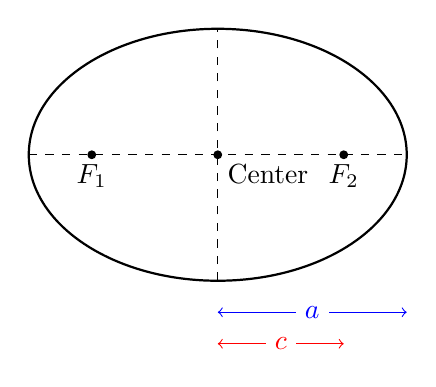
\begin{tikzpicture}[scale=0.8]
      % Draw the ellipse
      \draw[thick] (0,0) ellipse (3cm and 2cm);
      
      % Draw major and minor axes
      \draw[dashed] (-3,0) -- (3,0);
      \draw[dashed] (0,-2) -- (0,2);
      
      % Mark the center
      \fill (0,0) circle (2pt) node[below right] {Center};
      
      % Mark the foci
      \fill (-2,0) circle (2pt) node[below] {$F_1$};
      \fill (2,0) circle (2pt) node[below] {$F_2$};
      
      % Indicate the semi-major axis (a)
      \draw[<->, blue] (0, -2.5) -- (3, -2.5) node[midway, fill=white] {$a$};
      
      % Indicate the focal distance (c)
      \draw[<->, red] (0, -3.0) -- (2, -3.0) node[midway, fill=white] {$c$};
  \end{tikzpicture}
  \end{center}
  Additionally, the semi-minor axis $b$ is related to $a$ and $c$ by:
  
  \bigskip
  \textbf{Key Points:}
  \begin{itemize}
      \item If $e = 0$, the ellipse is a circle.
      \item If $0 < e < 1$, the ellipse is elongated, with greater elongation as $e$ increases.
  \end{itemize}
\end{frame}

\begin{frame}
  \frametitle{Hyperbola}
\begin{block}{Definition}
  The graph of the equation of the form 
  \[
\frac{y^2}{b^2} - \frac{x^2}{a^2} = 1
\]
where \(a,b\) are non-zero numbers
\end{block}
\end{frame}

\begin{frame}
  \begin{figure}
    \centering 
    \includegraphics[scale=0.5]{hyperbola2.png}
  \end{figure}
\end{frame}
\begin{frame}
  \frametitle{Hyperbola}
  \begin{block}{Foci}
    The foci of a hyperbola are two points with the property that the difference of
the distances from the foci to a point on the hyperbola is a constant independent
of the point on the hyperbola
  \end{block}
\end{frame}

\begin{frame}
  \begin{figure}
    \centering 
    \includegraphics[scale=0.4]{hyperbola3.png}
  \end{figure}
\end{frame}
\begin{frame}
  \begin{figure}
    \centering 
    \includegraphics[scale=0.5]{hyperbola1.png}
  \end{figure}
\end{frame}

\subsection{Exponents}
\begin{frame}
  \frametitle{Positive Integer Exponent}
  \begin{block}{Positive Integer Exponent}
    If \(x\) is a real number and \(m\) is a positive integer, then \(x^{m}\) is defined to be the
product with \(x\) appearing \(m\) times
\[x^{m} = \underset{x \;\;appears\;\;m \;\;times}{\underbrace{x \cdot x \cdots x }}\]
    
  \end{block}
\end{frame}

\begin{frame}
  \frametitle{Positive Integer Exponenets}
  \begin{block}{Properties}
    Suppose \(x\) and \(y\) are numbers and \(m\) and \(n\) are positive integers. Then 
    \[x^{m}x^{n} = x^{m+n} \]   
    \[\left(x^{m}\right)^{n} = x^{mn} \] 
    \[x^{m}y^{m} = \left(xy\right)^{m} \] 
  \end{block}
\end{frame}
\begin{frame}
  \frametitle{\(x^{0}\)} 
  \begin{alertblock}{What is \(x^{0}\)}
    If  \(x^{m}x^{n} = x^{m+n}\) then we can write \[x^{0}x^{n} = x^{0+n} = x^{n} \implies x^{0} = 1\;for\;\ x \neq 0\]
   \end{alertblock}

   \begin{alertblock}{What is \(0^{0}\)}
    \begin{itemize}
      \item The rule \( x^0 = 1 \) (for \( x \neq 0 \)) suggests that \( 0^0 \) should be \(1\).
      \item The rule \( 0^m = 0 \) (for \( m > 0 \)) suggests that \( 0^0 \) should be \(0\)
      \item Since these two rules contradict each other, \( 0^0 \) is left undefined in general mathematics.
      \item However, in combinatorics and programming, \( 0^0 \) is often defined as \(1\) for convenience.
  \end{itemize}
   \end{alertblock}
\end{frame}

\begin{frame}
  \frametitle{Negative Integer Exponents}
  If \(x^{m}x^{n} = x^{m+n}\), if we take \(m = -n \), then 
  \[x^{m}x^{-m} = x^{0} = 1 \implies x^{m}x^{-m} = 1\]
  We have to define \(x^{-m}\) to equal the multiplicative inverse of \(x^{m}\)
\begin{block}{Negative Interger Exponent}
  If \(x \neq 0\) and \(m\) is a positive integer, then \(x^{-m}\) is defined to multiplicative inverse of \(x^{m}\) 
  \[x^{-m} = \frac{1}{x^{m}}\]
  
\end{block}
\end{frame}

\begin{frame}
    \frametitle{Exponents: Some Graphs}
    \begin{columns}
      \begin{column}{0.5\textwidth}
        \begin{figure}
          \includegraphics[scale=0.4]{exponent-graph1.png}
          \caption{graph of \(\frac{1}{x}\)}
        \end{figure}
      \end{column}
      \begin{column}{0.5\textwidth}
        \begin{figure}
          \includegraphics[scale=0.4]{exponent-graph2.png}
          \caption{graph of \(\frac{1}{x^{2}}\)}
        \end{figure}
      \end{column}
    \end{columns}
\end{frame}
\begin{frame}
  \frametitle{Negative Integer Exponenets}
  \begin{alertblock}{Graph of Negative Integer Exponents}
    if \(m\) is  a positive integer then
    \begin{itemize}
      \item \(\frac{1}{x^{m}}\) behaves like \(\frac{1}{x}\) if \(m\) is odd
      \item \(\frac{1}{x^{m}}\) behaves like \(\frac{1}{x^{2}}\) if \(m\) is even
      \item Larger values of \(m\) correspond to functions whose graphs get closer to the x-axis more rapidly for large values of \(x\)
      and closer to the vertical axis more rapidly for values of \(x\) near 0
    \end{itemize} 
  \end{alertblock}  

\end{frame}

  \begin{frame}
    \frametitle{Roots}
    \begin{block}{\(m^{th}\) root}
   If \(m\) is a positive integer and \(x\) is a real number, then \(x^{1/m}\) is defined to be the real number satisfying the equation
   \[\left(x^{1/m}\right)^{m} = x \]
  subject to the following conditions:
  \begin{itemize}
    \item  If \(x < 0\) and \(m\) is an even integer, then \(x^{1/m} \)is undefined 
    \item If \(x > 0\) and \(m\) is an even integer, then \(x^{1/m} \) is chosen to be the \textit{\textcolor{red}{positive number}} satisfying the equation above
  \end{itemize}
The number \(x^{1/m}\) is called the \textbf{\(m^{th}\)} root of \(x\).
\end{block}
  
\end{frame}
\begin{frame}
  \frametitle{Roots}
  \begin{example}
    \begin{itemize}
      \item \(8^{1/3}\) and \(-8^{1/3}\)
      \item \(9^{1/2}\) and \(-9^{1/2}\)
    \end{itemize}
  \end{example}
  \begin{solution}
    \begin{enumerate}
      \item \( \left(8^{1/3}\right)^{3} = 8 \implies 2 \)
      \item \( \left(-8^{1/3}\right)^{3} = -8 \implies -2 \). There is no other number other than \(-2\)
      \item \( \left( 9^{1/2} \right)^{2} = -3 \; or \;3\). But as per the rule, we have to choose positive possibility, that is \(3\)
      \item \( \left( -9^{1/2} \right)^{2} \). No number real number exists so no solution 
    \end{enumerate}
  \end{solution}
\end{frame}


\begin{frame}{Rational Exponents}
  \begin{block}{Definition}
  Suppose \(\frac{n}{m}\) is a fraction in reduced form, where \(n\) and \(m\) are integers and \(m > 0\). Then, whenever it makes sense,
  \[
    x^{\frac{n}{m}} = \Bigl(x^{\frac{1}{m}}\Bigr)^n.
  \]
  \vspace{0.5em}
  \textbf{Note:} For the expression \(x^{\frac{1}{m}}\) to be defined, additional conditions on \(x\) may be required (for example, if \(m\) is even, then typically \(x \ge 0\)).
  \end{block}
\end{frame}

\begin{frame}{Algebra of Exponents}
  \begin{block}{Exponent Rules}
    Let \(p, q\) be rational numbers and \(x, y\) be positive numbers. Then the following rules hold:
    \begin{itemize}
      \item \(x^p \cdot x^q = x^{\,p+q}\)
      \item \(x^p \cdot y^p = (xy)^p\)
      \item \((x^p)^q = x^{\,pq}\)
      \item \(x^0 = 1\)
      \item \(x^{-p} = \dfrac{1}{x^p}\)
      \item \(\dfrac{x^p}{x^q} = x^{\,p-q}\)
      \item \(\left(\dfrac{x}{y}\right)^p = \dfrac{x^p}{y^p}\)
    \end{itemize}
  \end{block}
\end{frame}
\subsection{Polynomials}
\begin{frame}{Polynomial Definition}
  \begin{block}{Definition of a Polynomial}
    A polynomial is a function \( p \) such that
    \[
      p(x) = a_0 + a_1 x + a_2 x^2 + \cdots + a_n x^n,
    \]
    where \( n \) is a nonnegative integer and \( a_0, a_1, a_2, \dots, a_n \) are numbers.
  \end{block}
\end{frame}

\begin{frame}{Degree of a Polynomial}
  \begin{block}{Definition}
    Suppose \( p \) is a polynomial defined by
    \[
      p(x) = a_0 + a_1 x + a_2 x^2 + \cdots + a_n x^n.
    \]
    If \( a_n \neq 0 \), then we say that \( p \) has degree \( n \). The degree of \( p \) is denoted by \(\deg p\).
  \end{block}
\end{frame}


\begin{frame}{Polynomial Graphs}
  \centering
  % First Column
  \begin{minipage}[t]{0.45\textwidth}
    \centering
    \includegraphics[width=0.9\linewidth]{polynomial_degree_0.png}\\[1mm]
    \includegraphics[width=0.9\linewidth]{polynomial_degree_1.png}\\[1mm]
  \end{minipage}
  \begin{minipage}[t]{0.45\textwidth}
    \centering
    \includegraphics[width=0.9\linewidth]{polynomial_degree_2.png}
  \end{minipage}
\end{frame}


\begin{frame}
  \centering
  \begin{minipage}[t]{0.45\textwidth}
    \centering
    \includegraphics[width=\linewidth]{polynomial_degree_4.png}\\[1mm]
    \includegraphics[width=\linewidth]{polynomial_degree_7.png}
  \end{minipage}
\end{frame}


\begin{frame}{The Algebra of Polynomials}
  Two functions can be added, subtracted, or multiplied, producing another function. Specifically, if \(p\) and \(q\) are functions, then the functions 
  \[
    p+q,\quad p-q,\quad \text{and} \quad pq
  \]
  are defined by
  \[
    (p+q)(x) = p(x) + q(x),
  \]
  \[
    (p-q)(x) = p(x) - q(x),
  \]
  \[
    (pq)(x) = p(x) \, q(x).
  \]
\end{frame}


\begin{frame}{Degree of the Sum and Difference of Two Polynomials}
  \begin{alertblock}{Important Result}
  If \(p\) and \(q\) are nonzero polynomials, then
  \[
  \deg(p+q) \leq \max\{\deg p,\, \deg q\},
  \]
  and
  \[
  \deg(p-q) \leq \max\{\deg p,\, \deg q\}.
  \]
  \end{alertblock}

 
  \begin{alertblock}{Degree of the Product of Two Polynomials}
    If \(p\) and \(q\) are nonzero polynomials, then
    \[
    \deg(pq) = \deg p + \deg q.
    \]
  \end{alertblock}
\end{frame}


\begin{frame}{Example: Polynomials \(p\) and \(q\)}
  \begin{exampleblock}{Problem}
  Suppose \(p\) and \(q\) are polynomials defined by
  \[
  p(x) = 2 - 3x^2 \quad \text{and} \quad q(x) = 4x + 7x^5.
  \]
  Answer the following:
  \begin{enumerate}
      \item What is \(\deg p\)?
      \item What is \(\deg q\)?
      \item Find a formula for \(pq\).
      \item What is \(\deg(pq)\)?
  \end{enumerate}
  \end{exampleblock}
\end{frame} 
\begin{frame}
  \begin{exampleblock}{Solution}
  \begin{enumerate}
      \item Since \(p(x) = 2 - 3x^2\) has the highest power \(x^2\), we have \(\deg p = 2\).
      \item For \(q(x) = 4x + 7x^5\), the highest power is \(x^5\), so \(\deg q = 5\).
      \item The product \(pq\) is computed as follows:
      \[
      pq = (2-3x^2)(4x+7x^5) = 2\cdot 4x + 2\cdot 7x^5 - 3x^2\cdot 4x - 3x^2\cdot 7x^5,
      \]
      which simplifies to:
      \[
      pq = 8x - 12x^3 + 14x^5 - 21x^7.
      \]
      \item The highest power in \(pq\) is \(x^7\), so \(\deg(pq) = 7\).
  \end{enumerate}
  \end{exampleblock}
  \end{frame}


  \begin{frame}{Zeros/Roots of a Function}
    \begin{block}{Definition}
      A number \(t\) is called a zero of a function \(p\) if
      \[
        p(t) = 0.
      \]
    \end{block}
  \end{frame}

  \begin{frame}{Closed-Form Expression}
    \begin{block}{Definition}
      A closed-form expression is an explicit formula that can be written using a finite number of standard operations and functions (e.g., addition, multiplication, exponentiation, logarithms, trigonometric functions). It does not involve infinite series, integrals, or iterative processes.
    \end{block}
    \vspace{0.5em}
    \textbf{Example:} The quadratic formula,
    \[
      x = \frac{-b \pm \sqrt{b^2-4ac}}{2a},
    \]
    is a closed-form expression.
  \end{frame}
  
  \begin{frame}{Zeros of Higher–Degree Polynomials}
    \begin{block}{Key Points}
      \begin{itemize}
        \item The quadratic formula gives exact zeros for degree–2 polynomials.
        \item Although formulas exist for cubics and quartics, they are rarely used.
        \item No closed-form formula exists for polynomials of degree 5 or higher.
        \item Numerical methods can approximate zeros for any polynomial.
        \item \textbf{Example:} For 
        \[
          p(x)=x^5-5x^4-6x^3+17x^2+4x-7,
        \]
        approximate zeros are:
        \[
          -1.80,\; -0.73,\; 0.63,\; 1.48,\; 5.56.
        \]
      \end{itemize}
    \end{block}
  \end{frame}

\begin{frame}
  \frametitle{Zeros on graph}
  \centering
  \includegraphics[scale=0.23]{zeros.png}

\end{frame}

\begin{frame}
  \frametitle{Zeros on graph}
  \begin{columns}
    \begin{column}{0.5\textwidth}
      \centering
      \includegraphics[scale=0.3]{no-real-zeros.png}
    \end{column}
    \begin{column}{0.5\textwidth}
      The function \(x^{2}+1\) has no real zeros 
    \end{column}
  \end{columns}
\end{frame}

\begin{frame}{Factor of a Polynomial}
  \begin{block}{Definition}
    Suppose \(p\) is a polynomial and \(t\) is a real number. Then \(x-t\) is called a \emph{factor} of \(p(x)\) if there exists a polynomial \(G(x)\) such that
    \[
      p(x) = (x-t)\,G(x)
    \]
    for every real number \(x\).
  \end{block}
\end{frame}

\begin{frame}{Example: Factors and Zeros of a Polynomial}
  \begin{exampleblock}{Problem}
    Let 
    \[
      p(x) = (x-2)(x-5)(x^2+1).
    \]
    \begin{enumerate}[(a)]
      \item Explain why \(x-2\) is a factor of \(p(x)\).
      \item Explain why \(x-5\) is a factor of \(p(x)\).
      \item Show that \(2\) and \(5\) are zeros of \(p\).
      \item Show that \(p\) has no (real) zeros except \(2\) and \(5\).
    \end{enumerate}
  \end{exampleblock}
\end{frame}
\begin{frame}
  \begin{block}{Solution}
    \begin{enumerate}[(a)]
      \item The polynomial is given in factored form as \((x-2)(x-5)(x^2+1)\). Since \((x-2)\) appears as one of the factors, it is a factor of \(p(x)\).
      \item Similarly, \((x-5)\) appears explicitly in the factorization, so it is a factor of \(p(x)\).
      \item To show that \(2\) and \(5\) are zeros, substitute:
        \[
          p(2) = (2-2)(2-5)(2^2+1) = 0\cdot(-3)\cdot5 = 0,
        \]
        \[
          p(5) = (5-2)(5-5)(5^2+1) = 3\cdot0\cdot26 = 0.
        \]
        Thus, \(p(2)=0\) and \(p(5)=0\).
      \item The factor \(x^2+1\) yields \(x^2=-1\), which has no real solutions. Hence, aside from the zeros from \((x-2)\) and \((x-5)\), there are no other real zeros.
    \end{enumerate}
  \end{block}
\end{frame}

\begin{frame}{Zeros and Factors of a Polynomial}
  \begin{block}{Key Fact}
    Suppose \(p\) is a polynomial and \(t\) is a real number. Then \(t\) is a zero of \(p\) if and only if \(x-t\) is a factor of \(p(x)\).
  \end{block}
\end{frame}

\begin{frame}{Number of Zeros of a Polynomial}
  \begin{block}{Fundamental Property}
    A nonzero polynomial \(p(x)\) of degree \(n\) has at most \(n\) zeros.
  \end{block}

  \begin{block}{Explanation}
    A polynomial of degree 15 has at most 15 zeros. This is because each (real) zero \(t_j\) of a polynomial \(p\) corresponds to a factor \((x-t_j)\) in a factorization of the form
    \[
      p(x) = (x-t_1)(x-t_2)\cdots(x-t_m) \, G(x),
    \]
    where \(G(x)\) is a polynomial with no (real) zeros. If \(p(x)\) had more than 15 zeros, then the right-hand side would represent a polynomial of degree higher than 15, contradicting the fact that \(p\) is of degree 15.
  \end{block}
\end{frame}


\begin{frame}{Behavior of a Polynomial Near \(\pm\infty\)}
  \begin{block}{Key Concepts}
    \begin{itemize}
      \item \textbf{\(x\) near \(+\infty\):} \(x\) is very large.
      \item \textbf{\(x\) near \(-\infty\):} \(x\) is very negative (i.e., \(|x|\) is very large).
      \item Our goal is to determine whether a polynomial \(p(x)\) is positive or negative in these extremes.
    \end{itemize}
  \end{block}
\end{frame}

\begin{frame}
  \centering
  \includegraphics[scale=0.2]{at-infty.png}

%  \centering
%  \includegraphics[scale=0.2]{at-infty2.png}

\end{frame}
 

\begin{frame}{Behavior of a Polynomial Near \(\pm\infty\)}
  \begin{block}{Key Ideas}
    \begin{itemize}
      \item To analyze the behavior as \(x\to\pm\infty\), factor out the highest degree term.
      \item If \(c\,x^n\) is the highest degree term in \(p(x)\), then for very large \(|x|\), \(p(x)\) behaves like \(c\,x^n\).
    \end{itemize}
  \end{block}
\end{frame}
   

\begin{frame}{Zero in an Interval}
  \begin{block}{Intermediate Value Theorem}
    Suppose \(p\) is a polynomial and \(a, b \in \mathbb{R}\) with \(a < b\). If \(p(a)\) and \(p(b)\) have opposite signs, then there exists a number \(c \in (a, b)\) such that \(p(c)=0\).
  \end{block}
\end{frame}


\begin{frame}{Example 7: Zero in an Interval}
  \begin{exampleblock}{Problem}
    Let 
    \[
      p(x) = x^5 + x^2 - 1.
    \]
    Explain why \(p\) has a zero in the interval \((0,1)\).
  \end{exampleblock}
  
  \begin{block}{Solution}
    Evaluate the polynomial at the endpoints:
    \[
      p(0) = 0^5 + 0^2 - 1 = -1 \quad \text{and} \quad p(1) = 1^5 + 1^2 - 1 = 1.
    \]
    Since \(p(0) < 0\) and \(p(1) > 0\), by the Intermediate Value Theorem, there exists a \(c \in (0,1)\) such that \(p(c)=0\).
  \end{block}
\end{frame}

\begin{frame}{Zeros for Polynomials with Odd Degree}
  \begin{block}{Key Result}
    Every polynomial with odd degree has at least one real zero.
  \end{block}
  \vspace{0.5em}
  \begin{itemize}
    \item For a polynomial \(p(x)\) of odd degree, as \(x \to -\infty\), \(p(x)\) tends to \(-\infty\) (or \(+\infty\)) and as \(x \to \infty\), \(p(x)\) tends to \(+\infty\) (or \(-\infty\)).
    \item By the Intermediate Value Theorem, since \(p(x)\) changes sign, there exists at least one real number \(c\) such that \(p(c)=0\).
  \end{itemize}
\end{frame}

\begin{frame}{Graph of \(p(x)=x^4-4x^3-2x^2+13x+12\)}
  % \centering
  % \includegraphics[width=\textwidth]{polynomial_plots.pdf}
\end{frame}

\begin{frame}{Choosing an Appropriate Graphing Interval}
  \begin{block}{Key Concepts}
    \begin{itemize}
      \item When graphing a polynomial, choose an interval that displays its peaks, valleys, and asymptotic behavior.
      \item For the polynomial
      \[
        p(x)=x^4-4x^3-2x^2+13x+12,
      \]
      an interval that is too narrow (e.g., \([-2,2]\)) fails to show its behavior as \(|x|\) grows.
      \item An interval like \([-2,4]\) better reveals the local extrema (peaks/valleys) and the fact that for large \(|x|\), \(p(x)\) behaves like \(x^4\).
      \item Using an excessively large interval (e.g., \([-50,50]\)) may hide the local features due to scaling.
      \item \textbf{Conclusion:} The interval \([-2,4]\) provides a good balance to illustrate the key features of the graph.
    \end{itemize}
  \end{block}
\end{frame}

\subsection{Rational Function}
\begin{frame}{Rational Function}
  \begin{block}{Definition}
    A \emph{rational function} is a function \(r\) defined by
    \[
      r(x) = \frac{p(x)}{q(x)},
    \]
    where \(p(x)\) and \(q(x)\) are polynomials, with \(q(x) \neq 0\).
  \end{block}
\end{frame}

\begin{frame}{Domain of a Rational Function \& Example for \(r(x)\)}
  \begin{block}{General Rule}
    The domain of a rational function 
    \[
      \frac{p(x)}{q(x)}
    \]
    is the set of all real numbers where the expression makes sense. Since division by 0 is undefined, we exclude all zeros of \(q(x)\).
  \end{block}
\end{frame}

\begin{frame}
  \begin{exampleblock}{Example }
    \[r(x)=\frac{3x^5+x^4-6x^3-2}{x^2-9}\]
    Factor the denominator:
    \[
      x^2-9=(x-3)(x+3).
    \]
    Thus, \(r(x)\) is undefined at \(x=3\) and \(x=-3\). Hence, its domain is
    \[
      \{x\in\mathbb{R}: x\neq 3 \text{ and } x\neq -3\}.
    \]
  \end{exampleblock}
\end{frame}

\begin{frame}{}
  \begin{exampleblock}{Example}
    \[s(x)=\frac{x^3-6x+5}{x^4+9}\]
    The denominator \(x^4+9\) is always positive (since \(x^4\ge 0\) and \(9>0\)). Therefore, \(s(x)\) is defined for every real number. \\
    Domain of \(s(x)\) :
    \(
      \mathbb{R}
    \)
  \end{exampleblock}
\end{frame}

\begin{frame}{Advantages of Mixed Representation}
  \begin{block}{Mixed Representation}
    Expressing a rational function as a polynomial plus a proper rational function (one where the numerator's degree is less than the denominator's) is analogous to writing an improper fraction as an integer plus a proper fraction.
  \end{block}
  \vspace{0.5em}
  \begin{block}{Advantages}
    \begin{itemize}
      \item \textbf{Simplification:} It makes further operations (such as integration, differentiation, and partial fraction decomposition) easier.
      \item \textbf{Asymptotic Insight:} The polynomial part reveals the behavior of the function as \(x\to\pm\infty\), while the proper fraction (the remainder) tends to zero for large \(|x|\).
      \item \textbf{Clarity:} It separates the "whole" part from the "fractional" part, making the function's structure more transparent.
    \end{itemize}
  \end{block}
\end{frame}

\begin{frame}{Mixed Rational Function Representation}
  \begin{exampleblock}{Problem}
    Express
    \[
      \frac{x^5 + 6x^3 + 11x + 7}{x^2+4}
    \]
    in the form
    \[
      G(x) + \frac{ax+b}{x^2+4},
    \]
    where \(G(x)\) is a polynomial and \(a, b\) are constants.
  \end{exampleblock}
\end{frame}

\begin{frame}{Procedure for Dividing Polynomials}
  \begin{block}{Steps}
    \begin{enumerate}
      \item \textbf{Rewrite:} Express the highest-degree term in the numerator as a single term times the denominator, plus the necessary adjustment.
      \item \textbf{Simplify:} Use the rewritten numerator to simplify the quotient.
      \item \textbf{Iterate:} Repeat steps (1) and (2) on the remaining rational function until the degree of the numerator is less than the degree of the denominator or the numerator becomes 0.
    \end{enumerate}
  \end{block}
\end{frame}

\begin{frame}{Mixed Representation Example (Part 1)}
  \begin{exampleblock}{Problem}
    Express
    \[
      \frac{x^5+6x^3+11x+7}{x^2+4}
    \]
    in the form
    \[
      G(x)+\frac{ax+b}{x^2+4},
    \]
    where \(G(x)\) is a polynomial and \(a, b\) are constants.
  \end{exampleblock}
\end{frame}
\begin{frame}
  \begin{block}{Step 1: Eliminate the \(x^5\) Term}
    Notice that
    \[
      x^5=x^3(x^2+4)-4x^3.
    \]
    Therefore,
    \[
    \begin{aligned}
      x^5+6x^3 &= x^3(x^2+4)-4x^3+6x^3\\[1mm]
               &= x^3(x^2+4)+2x^3.
    \end{aligned}
    \]
    So we can write:
    \[
      \frac{x^5+6x^3+11x+7}{x^2+4}=x^3+\frac{2x^3+11x+7}{x^2+4}.
    \]
  \end{block}
\end{frame}

\begin{frame}{Mixed Representation Example (Part 2)}
  \begin{block}{Step 2: Eliminate the \(2x^3\) Term}
    Write
    \[
      2x^3=2x(x^2+4)-8x.
    \]
    Then,
    \[
    \begin{aligned}
      2x^3+11x+7 &= 2x(x^2+4)-8x+11x+7\\[1mm]
                  &= 2x(x^2+4)+(3x+7).
    \end{aligned}
    \]
    Thus,
    \[
      \frac{2x^3+11x+7}{x^2+4}=2x+\frac{3x+7}{x^2+4}.
    \]
  \end{block}
\end{frame} 
\begin{frame}
  \begin{block}{Final Mixed Representation}
    Combining the steps, we have:
    \[
      \frac{x^5+6x^3+11x+7}{x^2+4}=x^3+2x+\frac{3x+7}{x^2+4}.
    \]
  \end{block}
\end{frame}

\begin{frame}{Division Algorithm for Polynomials}
  \begin{block}{General Result}
    If \(p(x)\) and \(q(x)\) are polynomials with \(q(x) \neq 0\), then there exist unique polynomials \(G(x)\) and \(R(x)\) such that
    \[
      \frac{p(x)}{q(x)} = G(x) + \frac{R(x)}{q(x)},
    \]
    where either \(R(x)=0\) or \(\deg R < \deg q\). Equivalently, we can write
    \[
      p(x)=q(x)G(x)+R(x).
    \]
  \end{block}
\end{frame}


\begin{frame}{Division by \(x-t\) and Zeros of a Polynomial}
  \begin{block}{Special Case}
    Fix a real number \(t\) and let \(q(x)=x-t\). Since \(\deg q=1\), the remainder \(R(x)\) is a constant \(c\)(Because degree \(R < \)degree \(q\)). Thus, there exist a polynomial \(G(x)\) and a constant \(c\) such that
    \[
      p(x) = (x-t)G(x) + c.
    \]
    Evaluating at \(x=t\) yields \(p(t)=c\), so we can rewrite this as
    \[
      p(x) = (x-t)G(x) + p(t).
    \]
  \end{block}
  \vspace{0.5em}
  \begin{block}{Application to Zeros}
    \(t\) is a zero of \(p\) if and only if \(p(t)=0\), which happens precisely when
    \[
      p(x)=(x-t)G(x).
    \]
  \end{block}
\end{frame}

\begin{frame}{Behavior of a Rational Function Near \(\pm\infty\)}
  \begin{block}{General Approach}
    To determine the behavior of a rational function as \(x\to\pm\infty\), factor out the highest power of \(x\) in the numerator and the denominator.
  \end{block}
\end{frame} 
\begin{frame}
  \begin{block}{Example}
    Consider 
    \[
      r(x)=\frac{9x^5-2x^3+1}{x^8+x+1}.
    \]
    The highest degree in the numerator is \(x^5\) and in the denominator is \(x^8\). Factoring these out yields:
    \[
      r(x) \sim \frac{9x^5}{x^8}=\frac{9}{x^3}.
    \]
    As \(|x|\) becomes very large:
    \begin{itemize}
      \item \(r(x)\to 0\) as \(x\to\infty\) (approaching \(0^+\)).
      \item \(r(x)\to 0\) as \(x\to-\infty\) (approaching \(0^-\)).
    \end{itemize}
  \end{block}
\end{frame}

\begin{frame}{Asymptote of a Rational Function}
  \begin{block}{Definition}
    A line is an asymptote of a graph if the graph becomes and stays arbitrarily close to the line as \(x\) tends to \(\pm\infty\).
  \end{block}
  \vspace{0.5em}
  \begin{exampleblock}{Finding the Asymptote}
    Consider
    \[
      r(x)=\frac{3x^6-9x^4+6}{2x^6+4x+3}.
    \]
    Both the numerator and the denominator are degree 6. Therefore, the horizontal asymptote is the ratio of the leading coefficients:
    \[
      y=\frac{3}{2}.
    \]
  \end{exampleblock}
\end{frame}
\begin{frame}
  \begin{figure}
    \centering
    \includegraphics[scale=0.2]{asymptote1.png}
  \end{figure}
\end{frame}

\begin{frame}{Asymptote}
  \begin{exampleblock}{Example}
    \[
      r(x) = \frac{4x^{10}-2x^3+3x+15}{2x^6+x^5+1}
    \]
  \end{exampleblock}
  \begin{block}{Solution}
    \[
      \frac{4x^{10}}{2x^6} = 2x^4.
    \]
    Thus, as \(|x|\to\infty\), \(r(x)\) behaves like \(x^{4}\). That is, \(r(x)\) is very large and positive when \( x \to \infty\) and \( x \to -\infty\) 
  \end{block}
\end{frame}


\end{document}
   \section{Exponential Functions, Logarithms and e}

\begin{frame}{Bacterial Growth on the Human Body}
  \begin{itemize}
    \item Our skin (and other areas like the mouth, nose, and intestines) hosts hundreds of thousands of microscopic organisms.
    \item In fact, bacterial cells in our body outnumber our own cells.
    \item While some bacteria can cause illness, many are essential for our health.
    \item Bacteria reproduce through binary fission—each cell splits into two.
    \item Under ideal conditions, a single bacterium doubling every hour can lead to over 1,000 cells in 10 hours and more than 16 million in 24 hours.
  \end{itemize}
\end{frame}

\begin{frame}{Bacterial Growth Over Time}
  \begin{table}[ht]
    \centering
    \begin{tabular}{c|ccccccccccc}
      \textbf{Hour} & 0 & 1 & 2 & 3 & 4 & 5 & 6 & 7 & 8 & 9 & 10 \\ \hline
      \textbf{Bacteria} & 1 & 2 & 4 & 8 & 16 & 32 & 64 & 128 & 256 & 512 & 1024 \\
    \end{tabular}
    \caption{Bacterial cell count doubling every hour.}
  \end{table}
\end{frame}

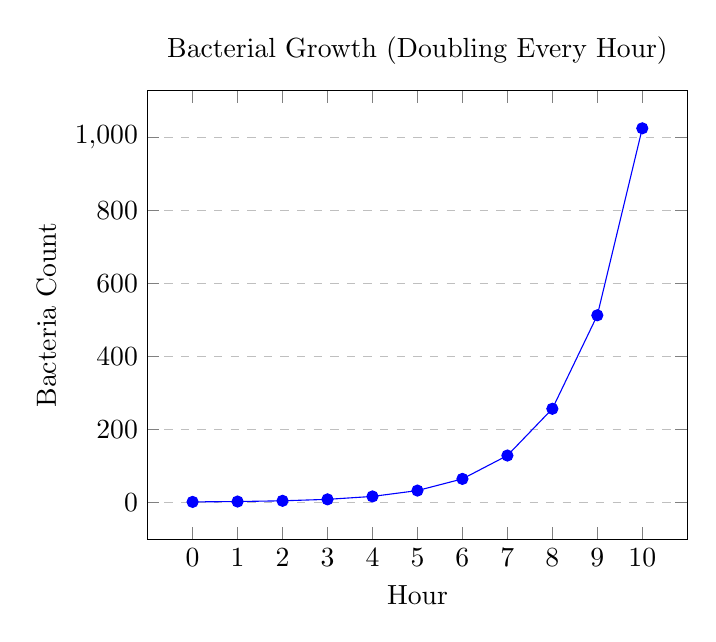
\begin{tikzpicture}
  \begin{axis}[
      xlabel={Hour},
      ylabel={Bacteria Count},
      title={Bacterial Growth (Doubling Every Hour)},
      xtick={0,1,2,3,4,5,6,7,8,9,10},
      ymajorgrids=true,
      grid style=dashed,
      % Uncomment the following line for a logarithmic scale on the y-axis:
      % ymode=log,
    ]
    \addplot[
      color=blue,
      mark=*,
      ]
      coordinates {
        (0,1) (1,2) (2,4) (3,8) (4,16) (5,32) (6,64) (7,128) (8,256) (9,512) (10,1024)
      };
  \end{axis}
\end{tikzpicture}

\begin{frame}{Population Growth in India}
  \begin{itemize}
    \item India is the second most populous country, with about 1.39 billion people in 2021.
    \item Its population grows at an annual rate of roughly 1.2\%.
    \item If this trend continues, India's population is projected to exceed China’s by 2027.
    \item While rapid population increases are often described as "exponential," in mathematics the term has a very precise meaning.
  \end{itemize}
\end{frame}

\begin{frame}{Defining Exponential Growth}
  \begin{block}{Key Concepts}
    \begin{itemize}
      \item \textbf{Percentage Change:} 
      \begin{itemize}
        \item refers to a change based on a percent of the original amount
      \end{itemize}
      \item \textbf{Exponential Growth:} 
        \begin{itemize}
          \item refers to an increase based on a constant multiplicative rate of change over equal increments of time, that is, a percent increase of the original amount over time.
          \item For example, if a quantity doubles each period, that is a 100\% increase per period.
        \end{itemize}
      \item \textbf{Linear Growth:} 
        \begin{itemize}
          \item The original value increases by a fixed \textbf{amount} (additive rate) over equal time intervals.
        \end{itemize}
        \item \textbf{Exponent Decay:}
        \begin{itemize}
          \item refers to a decrease based on a constant multiplicative rate of change over equal increments of time, that is, a percent decrease of the original amount over time.
        \end{itemize}
    \end{itemize}
  \end{block}
\end{frame}

\begin{frame}{Exponential Function and Its Behavior}
  \begin{block}{Definition}
    Suppose \(b>0\) with \(b\neq 1\). Then the \emph{exponential function} with base \(b\) is defined by
    \[
      f(x)=b^x.
    \]
    For example, if \(b=2\), then \(f(x)=2^x\). (Note that \(2^x\) is different from \(x^2\).)
  \end{block}
  \vspace{0.5em}
  \begin{block}{Behavior (for \(b>1\))}
    \begin{itemize}
      \item \textbf{Domain:} All real numbers, \(\mathbb{R}\).
      \item \textbf{Range:} All positive numbers, \((0,\infty)\).
      \item \(f(x)=b^x\) is an \emph{increasing} function.
      \item \(b^x\) becomes very large as \(x\) increases.
      \item \(b^x\) approaches \(0\) as \(x\) becomes very negative.
    \end{itemize}
  \end{block}
\end{frame}

\begin{frame}{Comparing Exponential and Linear Growth}
  \begin{table}[ht]
    \centering
    \begin{tabular}{c|c|c}
      \(x\) & \(f(x)=2^x\) & \(g(x)=2x\) \\ \hline
      0 & 1 & 0 \\
      1 & 2 & 2 \\
      2 & 4 & 4 \\
      3 & 8 & 6 \\
      4 & 16 & 8 \\
    \end{tabular}
    \caption{Exponential vs. Linear Growth.}
  \end{table}
  \begin{itemize}
    \item Linear growth (e.g., \(g(x)=2x\)) increases by a constant amount (2) for each increase in \(x\), that is, it is adding or subtracting a constant value. A constant amount \( \rightarrow \) linear growth or additive growth.
    \item Exponential growth (e.g., \(f(x)=2^x\)) increases by a constant factor (2) for each increase in \(x\), that is, it is multiplying or dividing by a constant value. A constant factor \( \rightarrow \) exponential growth or multiplicative growth.
  \end{itemize}
\end{frame}



\begin{frame}{Example: The Function \(f(x)=2^x\)}
  \begin{block}{Exponential Growth Illustrated (Table 2)}
    \begin{table}[ht]
      \centering
      \begin{tabular}{|c|c|c|c|c|c|c|c|}
        \hline
        \(x\)      & -3 & -2 & -1 & 0 & 1 & 2 & 3 \\ \hline
        \(2^x\) & \(2^{-3}=\frac{1}{8}\) & \(2^{-2}=\frac{1}{4}\) & \(2^{-1}=\frac{1}{2}\) & \(2^0=1\) & \(2^1=2\) & \(2^2=4\) & \(2^3=8\) \\ \hline
      \end{tabular}
      \caption{Exponential values of \(2^x\) for \(x=-3,\dots,3\).}
    \end{table}
  \end{block}
  \vspace{1em}
  \textbf{Observation:} As \(x\) increases by 1, the output of \(2^x\) doubles, clearly illustrating exponential growth.
\end{frame}




\begin{frame}{Algebraic Properties of Exponents}
  \begin{block}{Properties}
    Let \(a, b > 0\) and \(x, y \in \mathbb{R}\). Then:
    \begin{itemize}
      \item \(b^x \cdot b^y = b^{x+y}\)
      \item \((b^x)^y = b^{xy}\)
      \item \(a^x \cdot b^x = (ab)^x\)
      \item \(b^0 = 1\)
      \item \(b^{-x} = \dfrac{1}{b^x}\)
      \item \(\dfrac{b^x}{b^y} = b^{x-y}\)
      \item \(\dfrac{a^x}{b^x} = \Bigl(\dfrac{a}{b}\Bigr)^x\)
    \end{itemize}
  \end{block}
\end{frame}

\begin{frame}
  \frametitle{Exponent Graph}
  \begin{columns}
    \begin{column}{0.5\textwidth}
      \begin{figure}
        \centering 
        \includegraphics[scale=0.3]{exp-vs-poly1.png}
       \end{figure}      
    \end{column}
 

    \begin{column}{0.5\textwidth}
      \begin{figure}
        \centering 
        \includegraphics[scale=0.2]{exp-vs-poly2.png}
       \end{figure}      
    \end{column}
  \end{columns}
\end{frame}


  \begin{frame}{Logarithm}
    \begin{block}{Definition}
      Suppose \(b\) and \(y\) are positive numbers with \(b\neq 1\). 
      \begin{itemize}
        \item The logarithm base \(b\) of \(y\), denoted \(\log_b y\), is defined as the unique number \(x\) such that
        \[
          b^x = y.
        \]
        \item  Short Version
        \[
          \log_b y = x \quad \text{means} \quad b^x = y.
        \]
      \end{itemize}
    \end{block}
  \end{frame}

  \begin{frame}{Logarithm of 1 and the Base}
    \begin{block}{Key Properties}
      Let \(b>0\) with \(b\neq 1\). Then:
      \begin{itemize}
        \item \(\log_b 1 = 0\) because \(b^0 = 1\),
        \item \(\log_b b = 1\) because \(b^1 = b\).
      \end{itemize}
    \end{block}
  \end{frame}

  \begin{frame}{Logarithm as an Inverse Function}
    \begin{block}{Definition}
      Suppose \(b\) is a positive number with \(b \neq 1\) and the exponential function \(f\) is defined by
      \[
        f(x) = b^x.
      \]
      Then the inverse function \(f^{-1}\) is given by
      \[
        f^{-1}(y) = \log_b y.
      \]
    \end{block}
  \end{frame}
  
  \begin{frame}{Inverse Properties of Logarithms - Summary}
    \begin{itemize}
      \item \textbf{Inverse Relationship:}
        \begin{itemize}
          \item \(\log_b x\) is the inverse of \(b^x\).
          \item Flipping the graph of \(b^x\) across the line \(y=x\) yields the graph of \(\log_b x\).
        \end{itemize}
      \item \textbf{Monotonicity:}
        \begin{itemize}
          \item For \(b>1\), \(b^x\) is increasing, so \(\log_b x\) is also increasing.
        \end{itemize}
      \item \textbf{Key Equations:}
        \begin{itemize}
          \item \(b^{\log_b y} = y\)
          \item \(\log_b (b^x) = x\)
        \end{itemize}
      \item \textbf{Function-Inverse Properties:}
        \begin{itemize}
          \item These can be written as \((f \circ f^{-1})(y) = y\) and \((f^{-1} \circ f)(x) = x\).
        \end{itemize}
      \item \textbf{Understanding:}
        \begin{itemize}
          \item These properties are fundamental to the relationship between exponential and logarithmic functions.
        \end{itemize}
    \end{itemize}
  \end{frame}

  \begin{frame}{Logarithm of a Power}
    \begin{block}{Property}
      If \(b\) and \(y\) are positive numbers, with \(b \neq 1\), and \(t\) is a real number, then
      \[
        \log_b\left(y^t\right) = t \log_b y.
      \]
    \end{block}
  \end{frame}
\begin{frame}
  \frametitle{Radioactive Decay}
  If a radioactive isotope has half-life \(h\), then the function modeling the number of
  atoms in a sample of this isotope is
  \[ a(t) = a_{0}2^{-t/h}\]
  where \(a_{0}\) is the number of atoms of the isotope in the sample at time \(0\)
  \end{frame} 


  \begin{frame}
  \frametitle{Exponential Growth}
  \begin{block}{A story}
A mathematician in ancient India invented the game of chess. Filled with gratitude for the remarkable entertainment of this game, the king offered themathematician anything he wanted. The king expected the mathematician to
ask for rare jewels or a majestic palace.
But the mathematician asked only that he be given one grain of rice for the
first square on a chessboard, plus two grains of rice for the next square, plus
four grains for the next square, and so on, doubling the amount for each square,
until the 64th square on an 8-by-8 chessboard had been reached. The king was
pleasantly surprised that the mathematician had asked for such a modest reward.
A bag of rice was opened, and first 1 grain was set aside, then 2, then 4, then 8,
and so on. As the eighth square  was
reached, 128 grains of rice were counted out. The king was secretly delighted
to be paying such a small reward and also wondering at the foolishness of the
mathematician.
  \end{block}
  
  \end{frame}

  \begin{frame}
    \begin{block}{Story Cont..}
      As the 16th square was reached, 32,768 grains of rice were counted out—this
was a small part of a bag of rice. But the 21st square required a full bag of rice,
and the 24th square required eight bags of rice. This was more than the king had
expected. However, it was a trivial amount because the royal granary contained
about 200,000 bags of rice to feed the kingdom during the coming winter.
As the 31st square was reached, over a thousand bags of rice were required
and were delivered from the royal granary. Now the king was worried. By the
37th square, the royal granary was two-thirds empty. The 38th square would have
required more bags of rice than were left. The king then stopped the process
and ordered that the mathematician's head be chopped off as a warning about
the greed induced by exponential growth
    \end{block}
  \end{frame}
  \begin{frame}
    \frametitle{Mathematical analysis}
    \begin{itemize}
      \item \(64^{th}\) square requires \( 2^{63} \) grains \(\approx\) \(2^{3}* (2^{10})^{6} = 8*(10^{3})^{6} = 8*10^{18} \approx 10^{19} \) 
      \item if one large bag = \(10^{6} \) grains of rice , then total bags = \(10^{19}/10^{6} \) 
      \item In 2025 India's population is \(\approx 1 * 10^{9} \)
    \end{itemize}
     
    \end{frame}

    \begin{frame}
      \frametitle{Exponential Growth}
      \begin{block}{Definition}
      A function \(f\) is said to have \textbf{exponential growth} if \(f(x) = cb^{kx} \) where 
      \(c\) and \(k\) are positive numbers and \(b > 1\)
      \end{block}
      \begin{itemize}
        \item \(f(x) > p(x)\)  where \(f\) is exponenetial and \(p\) is polynomial for sufficiently large \(x\) 
        \item \(2^{x} > x^{1000} \)  \(\forall \;\; x > 13747 \)  
        \item A function \(f\) has exponential growth if and only if the graph of \(\log f(x)\) is a line with a positive slope
      \end{itemize}


    \end{frame}
    

    \begin{frame}
      \frametitle{Population Growth}
        \begin{block}{Exponential Growth}
          \[
            p(t) = p_0\,e^{rt}
          \]
          \begin{itemize}
            \item \(p_0\): initial population  
            \item \(r\): constant per-capita growth rate  
            \item Assumes unlimited resources → population grows without bound  
            \item Populations of various organisms, ranging from bacteria to humans, often exhibit exponential growth
          \end{itemize}
        \end{block}
    \end{frame}
    \begin{frame}
      \frametitle{Population Growth: Example}
      Suppose a colony of bacteria in a petri dish has 700 cells at 1 pm. These bacteria
      reproduce at a rate that leads to doubling every three hours. How many bacteria
      cells will be in the petri dish at 9 pm on the same day?
      \pause 
      \[
       p(t) = p_{0}2^{t/3} \implies 700 \cdot 2^{8/3} 
       \]
    \end{frame}


    \begin{frame} 
      \frametitle{Population Growth}
      \begin{block}{Exponential growth and doubling}
        If a population doubles every \( d \) time units, then the function \( p \) modeling this population growth is given by the formula

        \[
          p(t) = p_{0} \cdot 2^{(t-t_{0})/d}
        \]
        where \(p_{0}\) is the population at time \(t_{0}\)
        \end{block}    
    \end{frame}

    \begin{frame}
      \frametitle{Compound Interest}
      \begin{figure}
        \includegraphics[scale=0.3]{CI-comic.png}
      \end{figure}
    \end{frame}

    \begin{frame}
      \frametitle{Example}
      Suppose you deposit \(8000\) in a bank account that pays \(5\%\) annual interest. Assume the bank pays interest once per year at the end of the year, and that each year you place the interest in a cookie jar for safekeeping.
      \begin{enumerate}
        \item  How much will you have (original amount plus interest) at the end of two
        years?
        \item How much will you have (original amount plus interest) at the end of t years?
      \end{enumerate}
      \pause 
      Interest per year \( = 8000*0.05 = 400 \). For 2 years \( = 400*2 = 800\)

      After \(t\) years \(= 8000 + 8000*0.05*t = 8000(1+0.05t)\)
    \end{frame}

    \begin{frame}
      \frametitle{Simple Interest}
      \begin{block}{Simple Interest}
        If interest is paid once per year at the annual rate of \(r\), with no interest paid on the interest, then after \(t\) years 
        an initial amount \(P\) grows to 
        \[
           P(t) = P_{0}(1 + rt) 
        \]
        
      \end{block}
    \end{frame}

    \begin{frame}
      \frametitle{Example}
      Suppose you deposit \(8000\) in a bank account that pays \(5\%\) annual interest. Assume the bank pays interest once per year at the end of the year, and that each year the interest is deposited in the bank account
      \begin{enumerate}
        \item How much will you have at the end of one year?
        \item How much will you have at the end of two years?
        \item How much will you have at the end of t years?
      \end{enumerate}
      \pause 
      \begin{enumerate}
        \item  At the end of an year \( =  8000 + 8000*0.05  = 8400 \implies 8000(1+0.05)\)
        \item  At the end of 2 year \( = 8400 + 8400*0.05 \implies 8400( 1 + 0.05) = 8000(1.05)^{2} \) 
        \item  At the end of \(t\) years \(= 8000(1.05)^{t}\)
      \end{enumerate}
     
    \end{frame}

    \begin{frame}
      \frametitle{SI vs CI}
      \begin{figure}
        \includegraphics[scale=0.5]{SI_vs_CI.png}
      \end{figure}
    \end{frame}

    \begin{frame}
      \frametitle{Example}
\begin{itemize}
  \item Interest is often compounded more than once per year 
  \item In the above example,if the interest is compunded twice an year means instead of \(5\%\) being paid every year the interest comes as two payments of \(2.5\%\) each year with each payment made at the end of every 6 months
\end{itemize}
Suppose you deposit \(8000\) in a bank account that pays \(5\%\) annual interest, com-
pounded twice per year. How much will you have at the end of one year?

\pause 

\begin{itemize}
  \item At the end of 6 months \(= 8000(1+.025) \) 
  \item At the end of 1 year = \( (8000*1.025)(1.025) = (8000*1.05/2)^2 \)
  \item At the end of t years = \(8000*(1+\frac{0.05}{2})^{2*t} \)
\end{itemize}
\end{frame}
\begin{frame}
  \frametitle{Compound Interest}
  \begin{block}{\(n\) times per year}
    If the interest is compounded \(n\) times per year at annual interest rate
    \(r\) then after \(t\) years an initial amount of \(P_{0}\) grows to 

    \[P(t) = P_{0}(1+\frac{r}{n})^{nt}\]
    
  \end{block}
\end{frame}

\begin{frame}
  \frametitle{\( e \)}
  \begin{figure}
    \includegraphics[scale=0.5]{e_1.png}
  \end{figure}
\end{frame}

\begin{frame}
  \frametitle{area\((\frac{1}{x},1,2) < 1 \) }
  \begin{figure}
    \includegraphics[scale=0.8]{e_2.png}
  \end{figure}
  \begin{itemize}
    \item The area of the rectangle between \(x=1\) and \(x=2\) is \(1\) 
    \item The yellow region lies inside the rectangle and the area of the yellow region is less than \(1\) 
  \end{itemize}
\end{frame}



\begin{frame}
  \frametitle{area\((\frac{1}{x},1,3) > 1 \) }
  \begin{columns}
    \begin{column}{0.5\textwidth}
      \begin{itemize}
        \item Interval \([1, 3]\) divided into 8 equal parts; each has width \(\frac{1}{4}\).
        \item Heights are calculated using \(f(x) = \frac{1}{x}\) at left endpoints of subintervals.
        \item First three rectangles:
        \begin{itemize}
            \item 1st: Height = \(\frac{1}{\frac{5}{4}} = \frac{4}{5}\), Area = \(\frac{1}{4} \cdot \frac{4}{5} = \frac{1}{5}\)
            \item 2nd: Height = \(\frac{1}{\frac{7}{4}} = \frac{4}{7}\), Area = \(\frac{1}{4} \cdot \frac{4}{7} = \frac{1}{7}\)
            \item 3rd: Height = \(\frac{1}{\frac{9}{4}} = \frac{4}{9}\), Area = \(\frac{1}{4} \cdot \frac{4}{9} = \frac{1}{9}\)
        \end{itemize}
        \item Guess for all areas: \(\frac{1}{5}, \frac{1}{6}, \frac{1}{7}, \dots, \frac{1}{12}\)
        \item Total area: \(\sum_{k=5}^{12} \frac{1}{k} = \frac{28271}{27720} > 1\)
        
      \end{itemize}
    \end{column}
    \begin{column}{0.5\textwidth}
      \begin{figure}
        \includegraphics[scale=0.28]{e_3.png}
      \end{figure}
    \end{column}
  \end{columns}
\end{frame}

\begin{frame}
  \frametitle{Defining \(e\)}
  \begin{columns}
    \begin{column}{0.5\textwidth}
      \begin{itemize}
        \item Consider the area under \(y = \frac{1}{x}\) from \(1\) to \(c\).
        \item area\((\frac{1}{x},1,2^{2})\) = \(2*\text{area}(\frac{1}{x},1,2)\)
        \item area\((\frac{1}{x},1,3^{2})\) = \(2*\text{area}(\frac{1}{x},1,3)\)                 
        \item area\((\frac{1}{x},1,2^{3})\) = \(3*\text{area}(\frac{1}{x},1,2)\)
        \item In general, area\((\frac{1}{x},1,c^{t}) = t*\text{area}(\frac{1}{x},1,c)\) for every \(t>0\) and \(c>1\).
      \end{itemize}
    \end{column}
    \begin{column}{0.5\textwidth}
      \begin{tabular}{|c|c|}
        \hline
        \( c \) & \( \text{Area }( \frac{1}{x},1, c )\) \\
        \hline
        2 & 0.693147 \\
        3 & 1.098612 \\
        4 & 1.386294 \\
        5 & 1.609438 \\
        6 & 1.791759 \\
        7 & 1.945910 \\
        8 & 2.079442 \\
        9 & 2.197225 \\
        \hline
      \end{tabular}
    \end{column}
  \end{columns}
\end{frame}


\begin{frame}
  \frametitle{\(e \) }
  \begin{figure}
    \includegraphics[scale=0.5]{e_4.png}
  \end{figure}
\end{frame}

\begin{frame}
  \frametitle{Irrationality of \(e\)}
  \begin{itemize}
    \item The number \(e\) is irrational.
    \item Here is a 40-digit approximation of \(e\):
    \item \(e \approx 2.718281828459045235360287471352662497757\)
  \end{itemize}
\end{frame}

\begin{frame}
  \frametitle{Defining the Natural Logarithm}
  \begin{block}{Area under \(y = \frac{1}{x}\)}
      area\((\frac{1}{x},1,c^{t}) = t*\text{area}(\frac{1}{x},1,c) \)
  \end{block}
  \begin{itemize}
    \item The formula resembles the bhaviour of logarithms.
    \item Thus, area uner the curve \(y = \frac{1}{x}\) is connected with a logarithm
  \end{itemize}
  \[\text{area}(\frac{1}{x},1,e) = 1 \]
\[\text{area}(\frac{1}{x},1,e^{t}) = t \]

Assume \(t = \log_e c\) (the natural logarithm of \(c\)). Then we have
\[\text{area}(\frac{1}{x},1,c) = \text{area}(\frac{1}{x},1,e^{\log_e c}) = \log_e c\]  
\end{frame}


\begin{frame}
  \frametitle{Natural Logarithm}
  
      \begin{block}{Natural Logarithm}
        The natural logarithm, denoted \(\ln\), is defined as follows:
        \[
          \ln c = \log_e c
        \]
        for \(c > 1\).
      \end{block}
      \begin{figure}
        \centering
        \includegraphics[scale=0.35]{e_5.png}
      \end{figure}
\end{frame}

\begin{frame}
  \begin{block}{The exponenetial function}
    The \textbf{exponential function} is the function \(f\) defined by 
    \[ f(x) = e^{x} \]
    where \(e\) is the base of the natural logarithm.
  \end{block}
        \begin{itemize}
            \item The exponential function with base \( b \) is defined as \( b^x \).
            \item If no base is mentioned, assume the base is \( e \).
            \item The graph of \( e^x \) resembles \( 2^x \), \( 3^x \), etc., for \( b > 1 \).
            \item The function \(b^{x}\) is defined as \( b^{x} = e^{\ln b^{x}} \)
        \end{itemize}
\end{frame}

   \section{Trigonometric Functions}


\subsection{The Unit Circle}
\begin{frame}
    \frametitle{The Unit Circle}
\begin{definition}
    The \textbf{unit circle} is the circle in the Cartesian plane with center at the origin and radius 1, defined by the equation:
    \[
    x^2 + y^2 = 1
    \]
\end{definition}                                                                                                                                    
\end{frame}


 \begin{frame}
        \frametitle{Radius corresponding to a positive angle}
        \centering
        \includegraphics[scale=0.5]{/unit_circle/1.png}
    \end{frame}
    
    \begin{frame}
        \frametitle{Radius corresponding to a negative angle}
        \centering
        \includegraphics[scale=0.5]{/unit_circle/2.png}

    \end{frame}
    
    \begin{frame}
        \begin{block}{Positive and Negative Angles}
            \begin{itemize}
                \item Angle measurements for a radius on the unit circle are made from the
                positive horizontal axis.
                \item Positive angles correspond to moving counterclockwise from the positive
                horizontal axis.
                \item Negative angles correspond to moving clockwise from the positive hori-
                zontal axis.
            \end{itemize}
        \end{block}
    \end{frame}
    
    \begin{frame}
        \frametitle{Angles more than 360 degrees}
    \begin{block}{cyclic behaviour of angles}
        A radius of the unit circle corresponding to $\theta$ degrees also corresponds to
    $\theta + 360n$ degrees for every integer n.
    \end{block}
        \begin{figure}[h]    
            \centering
            \includegraphics[scale=0.4]{/unit_circle/3.png}
        \end{figure}
        
    \end{frame}
    


    \begin{frame}
        \frametitle{Length of a Circular Arc}
        \begin{figure}
            \centering
            \includegraphics[scale=0.5]{/unit_circle/5.png}
        \end{figure}
        \[ 360^{\circ}   \rightarrow  2 \pi r \implies \theta^{\circ}  \rightarrow \frac{\theta}{360}.2\pi r  = \frac{\theta \pi r}{180}\] 
    \end{frame}
    
    \begin{frame}
        \frametitle{Radians}
        For example an ant moving around a unit circle would travel a distance of $2\pi$ radians
        when it completes one full rotation.
       \begin{block}{Radians}
        Radians are a unit of measurement for angles such that $2\pi$ radians correspond
        to a rotation through an entire circle.
       \end{block}
    \end{frame}
    

    \begin{frame}
        \frametitle{Radians}
       \begin{block}{Degree to Radians}
    
        \[ 360^{\circ} = 2 \pi \text{ radians} \]
        \[ \theta ^{\circ}  = \frac{\theta \pi}{180} \text{ radians} \]
        
       \end{block}
    \end{frame}
    
    \begin{frame}
        \frametitle{Arc Length}
        \begin{block}{length of a circular arc}
            If $0 < \theta \leq 2\pi$ , then a circular arc on the unit circle corresponding to $\theta$ radians
            has length $\theta$         
        \end{block}
    \end{frame}

    \begin{frame}
        \frametitle{Area of a Sector}
        \begin{block}{Area of a sector}
            A sector/slice with angle $\theta$ radians inside a circle with radius $r$ has area $\frac{1}{2} \theta r^{2}$ .
        \end{block}
        \begin{figure}[h]    
            \centering
            \includegraphics[scale=0.25]{unit_circle/6.png}
        \end{figure}
    \end{frame}
    
    \begin{frame}
        \frametitle{Note}
        \begin{block}{Note}
            If no unit is specified, angles are assumed to be in radians.
        \end{block}
    \end{frame}

    \begin{frame}
        \frametitle{Cosine and Sine}
        \begin{block}{Definitions}
            \begin{itemize}
                \item The \textbf{cosine} of an angle $\theta$ is the x-coordinate of the point on the unit circle corresponding to that angle.
                \item The \textbf{sine} of an angle $\theta$ is the y-coordinate of the point on the unit circle corresponding to that angle.
            \end{itemize}
        \end{block}     
        \begin{figure}[h]    
            \begin{minipage}[b]{0.8\textwidth}
            \centering
            \includegraphics[scale=0.22]{unit_circle/7.png}
            \caption{sine and cosine}
        \end{minipage}
    \end{figure}
    \end{frame}

    \begin{frame}
        \frametitle{The Signs of Sine and Cosine} 
        \begin{figure}
            \centering
            \includegraphics[scale=0.2]{unit_circle/8.png}
            \caption{Signs of sine and cosine in different quadrants}
        \end{figure}
    \end{frame}

    \begin{frame}
        \frametitle{Key Equation Connecting Sine and Cosine} 
        \begin{itemize}
            \item By definition cosine and sine are the x and y coordinates of a point on the unit circle.
            \item The equation of the unit circle is $x^2 + y^2 = 1$.
            \item Therefore, for any angle $\theta$,
        \end{itemize}
        \begin{block}{Key Identity}
            \[\cos^2(\theta) + \sin^2(\theta) = 1\]
        \end{block}
    \end{frame}

    \begin{frame}
        \frametitle{The limits of Sine and Cosine} 
        \begin{itemize}
            \item For each real number $\theta$, there is a radius of the unit circle corresponding to that angle.
            \item The co-ordinates of the end point of the radius are $(\cos(\theta), \sin(\theta))$.
            \item That is this function is defined for all real numbers because theta can take any real value. 
            \item The domain of sine and cosine is all real numbers. \(\mathbb{R}\) 
            \item For unit circle \( \cos \theta^{2} + \sin \theta^{2} = 1 \) 
            \item Because \( \cos \theta^{2} + \sin \theta^{2} = 1 \) for all \(\theta\), the range of both sine and cosine is limited to \([-1, 1]\).
            \item 
        \end{itemize}
    \end{frame}



\end{document}